\documentclass[11pt]{article}
\usepackage[utf8]{inputenc}
\usepackage[T1]{fontenc}
\usepackage{lmodern}
\usepackage[a4paper,margin=2.5cm]{geometry}
\usepackage{amsmath,amssymb}
\usepackage{newunicodechar}
\usepackage{graphicx}
\usepackage{xltabular}
\usepackage{booktabs}
\usepackage{array}
\usepackage{enumitem}
\usepackage{tikz}
\usetikzlibrary{arrows.meta,positioning}
\usepackage[hidelinks]{hyperref}
\usepackage{xurl}
\setlist{nosep,leftmargin=*}
\setlength{\emergencystretch}{2em}
\renewcommand\tabularxcolumn[1]{>{\raggedright\arraybackslash\hspace{0pt}}p{#1}}
\newunicodechar{′}{\ensuremath{'}}
\newunicodechar{∧}{\ensuremath{\wedge}}
\newunicodechar{τ}{\ensuremath{\tau}}
\newunicodechar{σ}{\ensuremath{\sigma}}
\newunicodechar{β}{\ensuremath{\beta}}
\newunicodechar{ρ}{\ensuremath{\rho}}
\newunicodechar{λ}{\ensuremath{\lambda}}
\newunicodechar{κ}{\ensuremath{\kappa}}
\newunicodechar{ε}{\ensuremath{\varepsilon}}
\newunicodechar{×}{\ensuremath{\times}}
\newunicodechar{−}{\ensuremath{-}}
\newunicodechar{⪯}{\ensuremath{\preceq}}
\newunicodechar{⊆}{\ensuremath{\subseteq}}
\newunicodechar{⊂}{\ensuremath{\subset}}
\newunicodechar{→}{\ensuremath{\to}}
\newunicodechar{≥}{\ensuremath{\geq}}
\newunicodechar{≤}{\ensuremath{\leq}}
\newunicodechar{≠}{\ensuremath{\neq}}
\newunicodechar{≈}{\ensuremath{\approx}}
\newunicodechar{·}{\ensuremath{\cdot}}
\newunicodechar{…}{\ldots}
\newunicodechar{₀}{\textsubscript{0}}
\newunicodechar{₁}{\textsubscript{1}}
\newunicodechar{₂}{\textsubscript{2}}
\newunicodechar{₃}{\textsubscript{3}}
\newunicodechar{₇}{\textsubscript{7}}
\newunicodechar{ᵥ}{\textsubscript{v}}
\newunicodechar{ᵢ}{\textsubscript{i}}
\newunicodechar{ⱼ}{\textsubscript{j}}
\newunicodechar{ₖ}{\textsubscript{k}}
\newunicodechar{꜀}{\textsubscript{c}}

\title{Proofs, Attestation and Logs: What a Verifier Must Trust to Know a Safety Classifier Ran}
\author{Abdelhamid Bakhta, Lucid Computing (corresponding author)}
\date{}
\begin{document}
\maketitle

\begin{abstract}
Safety classifiers screen prompts and answers in many language-model services, yet users and auditors cannot check that the declared classifier produced the declared verdict on their request. We systematize operator-supplied evidence (self-report, black-box testing, replay, signed or logged records, statistical and refereed checks, hardware attestation, cryptographic proofs) by the trust elements each needs, and compare their trust sets by inclusion. Above the operator-reliant bottom class most pairs of classes are incomparable, and proofs sit above attestation only if proof-system soundness at the deployed parameters is counted with the other cryptographic assumptions and no setup is needed. Every compared class speaks to what was computed. Whether the verdict gated the answer, and when, needs a mechanism on the serving path that some attestation and logging designs supply and a proof cannot, so an auditor's order differs from the integrity order. The closest attested design attests a wrapper whose classifier runs outside it. We illustrate the systematization with Hallmark, an artifact the author built and ran, which proves synthetic threshold-classifier verdicts on a committed prompt of $\leq$96 bytes and a quantized TinyLlama-1.1B greedy answer, joined by a host check. There, residual trust sits in enrollment and host checks; for exact integer classifiers with public weights, replay needs less trust than the proofs; and the composition accepted classifier proofs made two days after the answer. The proofs spare a verifier the weights and re-execution; timings with unmatched boundaries show nothing about time. No proven security level, hiding, attestation or enforcement is claimed.

\medskip\noindent \textbf{Keywords:} evidence of execution; safety classifiers; trust assumptions; verifiable inference; succinct proofs; remote attestation; transparency logs; AI auditing
\end{abstract}

\section{Introduction}

Classifiers that screen the inputs and outputs of large language models (LLMs) are a common deployment layer. Llama Guard labels both the user prompt and the model response against a safety taxonomy \cite{D1}. Prompt Guard 2 classifies prompts as benign or malicious, and its smaller variant has 22 million parameters \cite{D6}. Rail frameworks and agent firewalls compose several such checks around one model \cite{D11}, \cite{D7}, at real cost: enhanced constitutional classifiers report a 23.7\% inference overhead relative to the base model \cite{D13}. The EU General-Purpose AI Code of Practice, which addresses providers of general-purpose AI models with systemic risk, lists ``monitoring and filtering the model's inputs and/or outputs'' as a mitigation (Safety and Security chapter, Measure 5.1) \cite{D24}, and signatories must document the implementation and limitations of their mitigations (Measure 7.3) \cite{D24}.

The party most affected by a guardrail cannot observe it. Under structured access, users and third parties reach a model only at arm's length, through an API or web interface \cite{D17}, and black-box access has been argued to be insufficient for rigorous audits \cite{D18}. This paper asks a narrow version of the verifiable-claims question \cite{D14}: what must a third-party verifier trust to accept that a specified classifier, with a specified threshold, computed a specified verdict on a specified LLM request?

Several kinds of evidence answer parts of that question. A verifier can replay the computation if determinism is engineered \cite{C1}, read a tamper-evident log \cite{C18}, run a statistical check \cite{C11}, rely on refereed delegation \cite{C10}, check a hardware attestation report \cite{B2}, or verify a proof of inference \cite{A5}, \cite{A17}. Two surveys compare some of these by verifiability: Peng et al. rate trusted execution environments and zero-knowledge proofs, among other techniques \cite{A32}, and Xia et al. score trusted execution, optimistic and zero-knowledge machine learning \cite{A35}. Neither includes replay or logs, and neither addresses guardrail verdicts. A clearing design for agentic commerce already orders evidence classes partially \cite{F9}; Section 6 states how our order differs. The closest same-question work, Proof-of-Guardrail by Jin et al., uses attestation: an Amazon Web Services (AWS) Nitro enclave runs a guardrail wrapper that calls Llama Guard 3-8B through the OpenRouter API, so the classifier itself runs outside the measured code. The attestation commits to the input and output, a user verifies it in about 5.1 ms, and the trust root is the cloud provider, whose Nitro hypervisor the authors trust to measure the code and protect the enclave's keys \cite{B24}.

The title's word ``ran'' needs care, because it can mean three things. A classifier \emph{computed} a verdict on the request; the verdict \emph{gated} the answer that was served; and it did so \emph{before} the answer was released. All the evidence classes we compare speak to the first reading. Only mechanisms that cover the serving path can speak to the other two, and Section 2.2 makes the distinction formal.

This is a systematization paper; the artifact serves as a worked illustration. We make four contributions.

\begin{enumerate}
\item \textbf{A statement-first account of what ``ran'' can mean} (Section 2). We separate the computation a classifier performed from whether its verdict gated the served answer and when, and record for every evidence class which of these it can speak to (Table 2).
\item \textbf{A systematization of evidence for that statement} (Sections 3 and 4). From a literature base collected by a stated procedure, we assign each evidence class the set of trust elements it needs and compare classes by inclusion of these sets (Table 1, Figure 1). Most of the resulting order is a direct reading of the assignments, and we say which results are. Its use is to make the assignments explicit, and to expose the edge readers most often assume, proofs over attestation, as conditional on how proof-system soundness and setup are assigned. Against the closest prior order \cite{F9}, it merges signed records with self-report and makes that edge conditional (Section 6).
\item \textbf{Three cross-cutting observations} (Section 4.4): the failure records of every class leave trust in some party or assumption, a claim the sets alone do not establish; request binding is a property of the statement, not of the class; and the integrity order differs from the order an auditor needs for gating and timing.
\item \textbf{A worked illustration and a gap analysis} (Sections 5 and 7). Hallmark proves synthetic classifier verdicts and a quantized LLM answer on one request. We use it to show where residual trust sits in one class-5 instance, and name compositions in the literature that could supply each property an auditor-ready receipt would still lack.
\end{enumerate}

\begin{center}\fbox{\parbox{0.94\linewidth}{\small \textbf{Box 1. Scope of the claims.} Hallmark's proofs are integrity proofs with public witnesses. They provide no zero-knowledge hiding (\texttt{hiding\_\allowbreak{}claim:\allowbreak{} false}) and no hardware attestation. They do not show that the prompt is what a real user sent, that the served answer depended on the verdict, or when the verdict was computed. No claim is made about whether verification is faster or slower than a native rerun (Section 5.4). The backend is not qualified (\texttt{qualified\_\allowbreak{}backend:\allowbreak{} false}), and no proven security level is stated (Section 5.3). Training is not proved. The three classifiers are synthetic: the frozen multilayer perceptron (MLP) allows every admitted input, and the convolutional neural network (CNN) blocks the benign prompt of the composed demonstration. Hallmark is a research artifact, built and run by the author, not a deployment. Jin et al. state that an attested guardrail ``should not be interpreted or advertised as proof-of-safety'' \cite{B24}, and the same holds here. Evidence that a guardrail ran says nothing about whether its decisions are adequate \cite{E2}. Later sections refer to this box rather than repeating it.}}\end{center}

Section 2 fixes the statement and threat model, Section 3 the literature base, and Section 4 the order; Section 5 works through Hallmark, Section 6 reviews related work, Section 7 lists gaps and limitations, and Section 8 concludes.

\section{Setting and Threat Model}

\subsection{Roles}

Three roles recur in every evidence class. The \emph{operator} serves the LLM, runs the guardrail and produces whatever evidence is offered. The \emph{verifier} checks that evidence; it may be the user who sent the request, an auditor, or a regulator acting for the user. The \emph{enroller} fixes, ahead of time, the reference identities against which evidence is compared: classifier, threshold, model and circuit. Among the roles of the Remote ATtestation procedureS (RATS) architecture (Attester, Verifier, Relying Party, Endorser and Reference Value Provider), Endorsers vouch for the Attester's authenticity, Reference Value Providers supply the values evidence is appraised against, and appraisal is a policy decision \cite{B5}. The enroller corresponds to the Reference Value Provider; applying these roles outside attestation is our framing. In Hallmark the caller is both enroller and verifier. Which institution should enroll in practice, and what that choice does to the trust placed in enrollment, is left to future work.

\subsection{The statement, and what ``ran'' means}

Evidence is always evidence \emph{of} something, so we fix the statement first. Let

\begin{center}\fbox{\parbox{0.94\linewidth}{\small S = ``classifier C, with threshold t, produced verdict V on request R, and model M produced answer Y on R''.}}\end{center}

C and M are identified by their enrolled descriptions (weights, architecture, arithmetic). R is the exact byte or token sequence the classifier and the model consumed. We distinguish six properties and record all but adequacy (Section 2.4) for each evidence class. The order of Section 4.1 concerns only the trust behind the first; the others are recorded as separate columns.

\begin{itemize}
\item \textbf{Integrity.} V is the value that C and t compute on R, and Y is the value that M computes on R.
\item \textbf{Request binding.} The evidence names R, so a verifier holding R accepts it and a verifier holding any R′ ≠ R rejects it.
\item \textbf{Hiding.} What the verifier learns about R and about the weights of C and M beyond S itself.
\item \textbf{Capture provenance.} R is the request the user actually sent, not one chosen by the operator.
\item \textbf{Adequacy.} C's verdicts implement a useful safety policy.
\item \textbf{Enforcement and timing.} The served answer Y depended on V, so that a block verdict withholds Y, and V was computed before Y was released.
\end{itemize}

S is a conjunction of two computations, with no gating clause and no temporal clause. Evidence for S therefore establishes what was computed: the first reading of ``ran'' in Section 1. A verifier who wants to know that a classifier ran in the sense of screening the served request needs a stronger statement,

\begin{center}\fbox{\parbox{0.94\linewidth}{\small S′ = S ∧ G ∧ T, where G says that Y was released only if V allowed it, and T says that V was computed before Y was released.}}\end{center}

G and T concern the serving path, not the two functions. Evidence for S′ must come from a mechanism that observes or controls that path. Section 4 records, for each class, whether it can.

Request binding is defined on the statement, not on the mechanism (Section 4.4). The statement must also say which verdict is meant, since guardrails such as WildGuard return several judgements \cite{D9}. S therefore names the head and the threshold as part of C: an operator that moves t changes verdicts without changing any weight.

S describes an input rail. An output rail computes its verdict on the answer, or on the request and the answer together, V = C(R, Y), and S changes accordingly. Nothing in Sections 2 to 4 depends on which input C reads, except T: an output verdict exists only after Y does, so T must then say that V was computed before Y was released to the user, not before Y was generated. Under streaming release Y leaves the operator piece by piece, and G and T concern every released prefix, which a mechanism on the serving path would have to hold back or check before release. Hallmark does not address streaming, and we leave it outside the systematization (Section 2.4). Two further details are implicit in S. R is the complete input the classifier consumed, including any conversation context and system prompt. And for sampled rather than greedy decoding, S must also bind the randomness from which Y was sampled, committed before generation.

\subsection{Adversary}

The adversary is the operator. It controls the serving infrastructure, chooses which evidence to produce and when, and wants a verifier to accept S when S is false. Its strategies are:

\begin{enumerate}
\item \textbf{Skip.} Do not run C, and report an allow verdict.
\item \textbf{Swap.} Run a different classifier C′ or threshold t′.
\item \textbf{Substitute.} Serve the answer of a cheaper model M′. Distribution-level tests detect this behind commercial APIs \cite{C14}, and output-only tests need many queries and miss subtle substitutions \cite{C15}.
\item \textbf{Replay.} Present evidence computed on a different request R′.
\item \textbf{Misreport.} Present a verdict V′ that C did not produce on R.
\item \textbf{Ignore.} Run C honestly on R, obtain V = block, and serve Y anyway.
\item \textbf{Defer.} Serve Y without running C on the live path, and compute C, and any evidence, later and only if a verifier asks.
\end{enumerate}

An evidence class defends against a strategy if, under its trust assumptions, the strategy makes verification fail. The verifier is honest and holds R, because it sent R or because R was disclosed to it. The enroller is honest and completes enrollment before any proof or report is produced. A misconfigured pipeline that silently bypasses a rail leaves the verifier with the same missing evidence as a deliberate skip. The systematization therefore supports detecting missing evidence, not attributing intent. A declared degraded mode, such as a classifier timeout that fails open, is likewise indistinguishable from Skip unless S names an enrolled fallback policy and the evidence records, before release, that the fallback was taken. Ignore and Defer differ from the first five strategies: every computation stays honest, and what breaks is G or T. Evidence for S cannot defend against them; only evidence for S′ can.

\subsection{Out of scope}

Four questions are outside the systematization. \emph{Adequacy}: formal checks find safety holes in all the guardrail classifiers they study \cite{E2}, and no evidence of execution repairs that. \emph{Side channels and physical attacks} on the verifier's own machine. \emph{Availability}: an operator can always refuse to serve evidence, and a verifier can only treat missing evidence as failure. \emph{Streaming release}, for the reasons given in Section 2.2.

\section{How the Literature Base Was Built}

The systematization rests on a literature base collected in four strands, one per family of mechanisms: (A) proofs of machine-learning inference and the proof systems beneath them; (B) hardware attestation and confidential computing; (C) replay, determinism, signed and transparency logs, and refereed, optimistic and statistical verification; and (D) the guardrail landscape, assurance literature and governance texts. Each strand was searched on 2026-10-30 with public topic terms in web search and on primary pages (arXiv, the Cryptology ePrint Archive of the International Association for Cryptologic Research (IACR), venue proceedings, standards bodies, official repositories), with follow-up searches for same-question work and, during revision, for sources reviewers named. A source was included if it describes a mechanism that produces evidence about the integrity of an inference or a record of it, reports a failure of such a mechanism, or states a governance demand for such evidence. Every source was opened on a primary page or metadata endpoint, and its annotation records trust root, request binding, hiding, verifier cost and failure mode as the source states them.

Reading depth varies, and we report it. Before review, an integrity check of this manuscript re-read the cited passages from source full texts for 69 of the 81 references then cited. Among the sources used to place a system in a class, the following were checked at abstract or title level only: the prompt binding of DeepProve \cite{A17}, ZKML \cite{A8}, Sigstore \cite{C20}, and the audit-framing works \cite{D16}, \cite{D18}. Proof-of-Guardrail \cite{B24} was read in full during revision, which changed its description (Section 4.3). Sources added in the final revision at reviewers' request (\cite{A39}, \cite{A40}, \cite{A41}, \cite{A42}, \cite{A43}, \cite{B25}, \cite{B26}) were checked on their primary pages for the specific statements cited; for \cite{A43} only the ePrint record, which gives its title and scope, could be retrieved; Seal-then-sample \cite{A22} was re-read for its setup. Class assignments of systems we did not run come from their own descriptions and may err in either direction.

\section{Evidence Classes Ordered by Trust}

\subsection{Trust universe and order}

Peng et al. rate the verification capability of trusted execution environments (TEEs) as ``Limited (attestation)'' and of zero-knowledge proofs as ``Strong'' \cite{A32}; Xia et al. score verifiability as 5 for zero-knowledge machine learning (zkML), 3 for optimistic machine learning (opML) and 2 for TEEs, and count trusted parties: ``zkML requires 0 trusted parties (only mathematical assumptions)'', opML at least one honest challenger and TEEs the hardware manufacturer \cite{A35}. We turn their scalar axes into a relation over a set U of trust elements on which evidence for the integrity of S can rest:

\begin{itemize}
\item \emph{O}, the operator's honesty;
\item \emph{E}, correct enrollment of reference identities \cite{B5};
\item \emph{P}, a correct implementation of C and M, whether in the verifier's code, a delegated program, a measured image or a circuit \cite{A23}, \cite{A30};
\item \emph{K}, cryptographic assumptions (hashes, signatures, commitments and proof-system soundness) at the deployed parameters \cite{A24}, \cite{A28};
\item \emph{N}, an honest participant in the ceremony that generated a structured reference string, for proof systems that need one \cite{A41}, \cite{A42};
\item \emph{D}, deterministic execution \cite{C1}, \cite{C10};
\item \emph{H}, one honest replica or challenger, online when needed \cite{C6}, \cite{C9};
\item \emph{T}, empirical soundness of a tolerance check \cite{C11}, \cite{C12};
\item \emph{Q}, unpredictability of what is sampled or challenged, including, for secret-based checks, the secrecy of the verifier's secret \cite{C12}, \cite{C13};
\item \emph{W}, the attestation root: the hardware, firmware and keys of whoever signs the attestation. W has three instances. For CPU TEEs it is a silicon vendor (\emph{W}\_v) \cite{B2}. GPU TEEs add NVIDIA's keys (\emph{W}\_g) to the CPU vendor's, since H100 confidential computing relies on a CPU TEE \cite{B6}, so a GPU TEE needs strictly more trust than a CPU TEE alone, a refinement within class 4 that the class-level order does not draw. For AWS Nitro Enclaves it is the cloud provider's hypervisor and keys (\emph{W}\_c) \cite{B24}.
\end{itemize}

Each class X has a trust set τ(X) ⊆ U (Table 1). Define X ⪯ Y, read ``Y needs no more trust than X'', to hold if and only if τ(Y) ⊆ τ(X). Inclusion is reflexive and transitive, so ⪯ is a preorder. It is not antisymmetric on classes, because self-report and signed records receive the same set. Its quotient, which merges classes with equal trust sets, is a partial order; we call the preorder \emph{the order}, and Figure 1 draws its quotient. Two modelling choices fix the bottom and the shared elements. Because O is the adversary, evidence whose integrity relies on O is no evidence against it, so we assign such a class the whole universe, τ = U, a convention that places operator-reliant classes at the bottom by construction. And E is assumed for every class, P for every class that checks a computation. The order compares classes; Result 5 below refines it by the computation and by what the verifier holds, and is not a relation between classes.

\subsection{What the order says}

The order has four unconditional results and a refinement. Results 1 to 4 are readouts of Table 1, not discoveries: E and P are shared by convention, the bottom is placed by convention, and the classes above the bottom differ by elements of their own (T and Q for 3a, H for 3b, W for 4, D for replay and 3b), so both the incomparabilities and the edges into proofs, whose set \{E, P, K\} each of 3a, 3b and 4 contains, follow from the assignments. We state them because the assignments carry the content, and a reader who disputes one can see which result changes.

\begin{enumerate}
\item Self-report (0a) and signed or logged records (2) rely on O and form the bottom class. Black-box testing (0b) binds no request and is not compared.
\item Replay (1), with τ = \{E, P, D\}, needs no more trust than refereed delegation (3b), with τ = \{E, P, K, D, H\}. Replay spares the verifier K and an honest party, at the price of a rerun.
\item Statistical checks (3a), refereed delegation (3b) and attestation (4) are pairwise incomparable. A verifier who distrusts the attestation root prefers 3b to 4; one who cannot ensure an honest challenger is online prefers 4 to 3b.
\item Replay and proofs (5), with τ = \{E, P, K\}, are incomparable in general: one needs D, the other K.
\item \emph{A refinement, not a class relation.} When the computation is an exact integer program and the verifier holds the weights, D holds by construction. Replay of that computation then needs only \{E, P\}, less than every other class, proofs included. Section 5.4 meets this case.
\end{enumerate}

Of the 21 pairs among the seven compared classes, 15 are comparable with the dashed edges of Figure 1 and 12 without them; all but four comparable pairs (one without the dashed edges) involve the bottom class. Among the five classes above the bottom, 6 of the 10 pairs are incomparable with the dashed edges and 9 without.

The three edges from 3a, 3b and 4 into 5 are conditional: they hold only because K places proof-system soundness at the deployed parameters in one class with the hash, signature and commitment assumptions the other classes already need. A verifier who separates the two finds 5 incomparable with 3a, 3b and 4, directly above the bottom class, and that separation is reasonable whenever the parameters carry no proven security level, as for Hallmark (Section 5.3). Proof systems whose polynomial commitments need a structured reference string, such as KZG commitments \cite{A41}, also need N, and for them the three edges fail even when soundness is counted within K. The order thus supports no claim that proofs dominate attestation: proofs replace W with proof-system soundness, and possibly N, and whether that is an improvement depends on parameters and setup the order does not weigh. Figure 1 draws both readings with equal weight.

Class numbers are kept only as short keys for the tables, not heights, and the order is not a ladder: replay (class 1) needs less trust than refereed delegation (class 3b). Like the graded levels of the Supply-chain Levels for Software Artifacts (SLSA) specification \cite{C23}, the order is a vocabulary for stating what evidence rests on, not a recommendation. Hybrids are compositions, not new classes: Slalom pairs a TEE with Freivalds checks \cite{B11}, Atlas a TEE with transparency logs \cite{C24}, and Seal-then-sample \cite{A22} and IMMACULATE \cite{C13} pair proofs with sampled coverage (5 + 3a).

\begin{figure}[htbp]
\centering
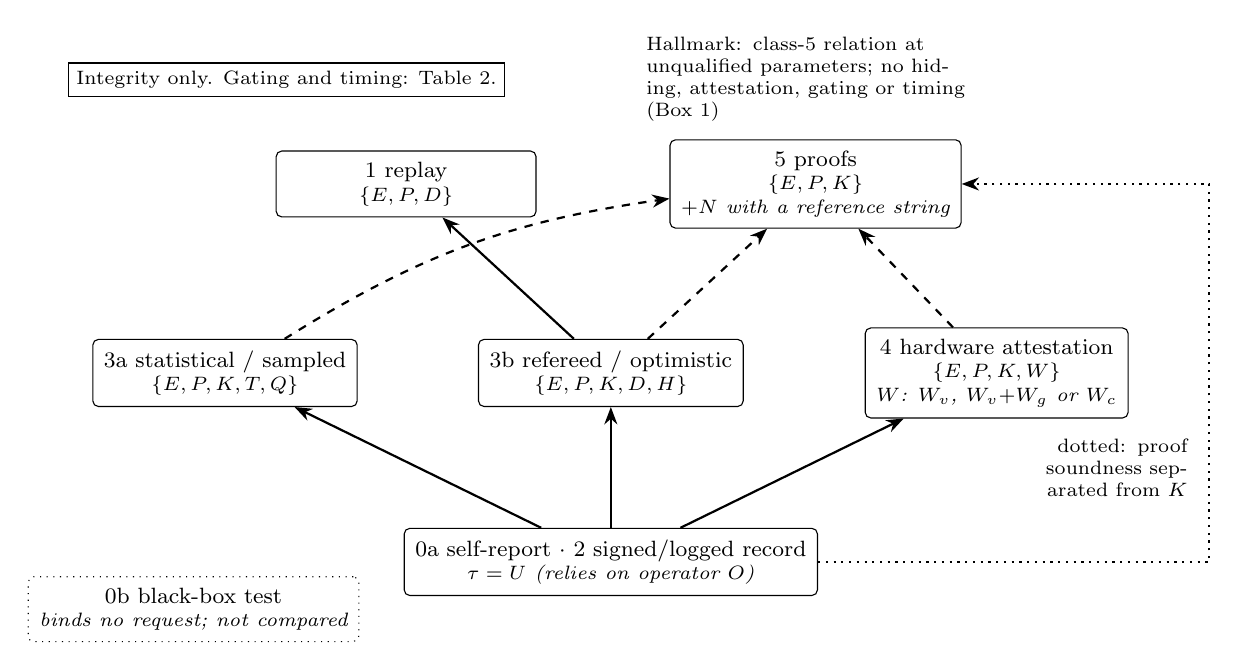
\begin{tikzpicture}[
  cls/.style={draw, rounded corners=2pt, align=center, font=\footnotesize, inner sep=4pt, minimum width=3.3cm},
  note/.style={font=\scriptsize, align=left, text width=4.3cm},
  edge/.style={-{Stealth[length=2.2mm]}, thick},
  cond/.style={edge, dashed},
  alt/.style={edge, dotted},
]
\node[cls] (N0) at (0,0) {0a self-report $\cdot$ 2 signed/logged record\\[-1pt]{\scriptsize\itshape $\tau = U$ (relies on operator $O$)}};
\node[cls] (N3a) at (-4.9,2.4) {3a statistical / sampled\\[-1pt]{\scriptsize\itshape $\{E,P,K,T,Q\}$}};
\node[cls] (N3b) at (0,2.4) {3b refereed / optimistic\\[-1pt]{\scriptsize\itshape $\{E,P,K,D,H\}$}};
\node[cls] (N4) at (4.9,2.4) {4 hardware attestation\\[-1pt]{\scriptsize\itshape $\{E,P,K,W\}$}\\[-1pt]{\scriptsize\itshape $W$: $W_v$, $W_v{+}W_g$ or $W_c$}};
\node[cls] (N1) at (-2.6,4.8) {1 replay\\[-1pt]{\scriptsize\itshape $\{E,P,D\}$}};
\node[cls] (N5) at (2.6,4.8) {5 proofs\\[-1pt]{\scriptsize\itshape $\{E,P,K\}$}\\[-1pt]{\scriptsize\itshape $+N$ with a reference string}};
\node[cls, dotted] (N0b) at (-5.3,-0.6) {0b black-box test\\[-1pt]{\scriptsize\itshape binds no request; not compared}};
\draw[edge] (N0) -- (N3a);
\draw[edge] (N0) -- (N3b);
\draw[edge] (N0) -- (N4);
\draw[edge] (N3b) -- (N1);
\draw[cond] (N3a) to[bend left=12] (N5);
\draw[cond] (N3b) -- (N5);
\draw[cond] (N4) -- (N5);
\draw[alt] (N0.east) -| (7.6,4.8) -- (N5.east);
\node[anchor=east, font=\scriptsize, text width=2.6cm, align=right] at (7.45,1.2) {dotted: proof soundness separated from $K$};
\node[note, above=1mm of N5] {Hallmark: class-5 relation at unqualified parameters; no hiding, attestation, gating or timing (Box~1)};
\node[draw, font=\scriptsize, anchor=south west, inner sep=3pt] at (-6.9,5.9) {Integrity only. Gating and timing: Table~2.};
\end{tikzpicture}
\caption{Evidence classes ordered by inclusion of trust sets (the quotient of the order; integrity of the statement only). An arrow from $X$ up to $Y$ means $\tau(Y)\subseteq\tau(X)$: $Y$ needs no more trust than $X$. Only cover edges are drawn, and class numbers are labels, not heights. Two readings are drawn with equal weight. Dashed edges into class~5 hold only if proof-system soundness at the deployed parameters is counted within $K$ and no setup ceremony ($N$) is needed; if soundness is separated, class~5 is covered directly by the bottom class (dotted edge) and sits level with 3a, 3b and 4, so its drawn height follows the dashed reading for layout only. Replay (1) and proofs (5) are incomparable, as are 3a, 3b and 4. For Proof-of-Guardrail (class~4), $W=W_c$ (AWS) and the classifier verdict is computed by an external API outside the measurement. Gating and timing (Table~2) order the classes differently.}
\label{fig:order}
\end{figure}



\subsection{The classes}

\textbf{Class 0: self-report (0a) and black-box testing (0b).} A model card or safeguard report is written by the developer about its own system \cite{C25}, \cite{D23}; the verifier trusts the author, and nothing binds the document to a request. A two-sample test can tell from output distributions whether an API serves a reference model, with a median power of 77.4\% at an average of 10 samples per prompt \cite{C14}, but it binds no request and can be evaded by routing audit traffic differently \cite{C15}, so it is an external check on self-report, outside the order.

\textbf{Class 1: replay.} The verifier re-executes the classifier or model on R and compares results. For floating-point LLM serving this works only when determinism is engineered: with batch-invariant kernels, 1,000 completions were identical, against 80 distinct completions by default \cite{C1}; otherwise outputs vary with batch size, GPU count and GPU type \cite{C2} and across runs of hosted APIs \cite{C3}. The verifier must hold the enrolled weights and match the operator's configuration \cite{C1}, \cite{C4}. We infer that replay binds only the input the verifier replays, not the request the operator served.

\textbf{Class 2: signed or transparency-logged records.} A signed, append-only record shows that a key holder wrote an entry and did not later alter or fork it, not that the logged event was computed correctly \cite{C16}, \cite{C18}. For a guardrail record the writer is the operator, and permanence also rests on auditors that compare views \cite{C17}; with keyless signing, the signer's identity also rests on the OpenID Connect identity provider \cite{C20}. A log binds the claim, not the computation \cite{C17}, but it can add time: an entry written before the answer is released fixes the claimed verdict at that moment.

\textbf{Class 3a: statistical or sampled checks.} The operator commits to intermediate signals, which the verifier checks against the claimed model and prompt within a tolerance. TOPLOC, a locality-sensitive hashing scheme, reports no false positives or negatives in its authors' tests, at 258 bytes per 32 new tokens for Llama 3.1-8B-Instruct, with empirical rather than cryptographic soundness \cite{C11}; SVIP is secret-based: it uses a learned identifier with non-zero error rates and a secret that the provider must not learn \cite{C12}. IMMACULATE audits a sampled fraction of requests using verifiable computation, so unaudited requests carry no proof \cite{C13}; like Seal-then-sample, it composes class 5 with sampling.

\textbf{Class 3b: refereed or optimistic delegation.} The result is correct if at least one server or challenger is honest \cite{C6}, \cite{C10}; optimistic schemes also need that party online within a challenge window \cite{C8}, \cite{C9}. Binding to the delegated program and input is native, the happy path is cheap, and a dispute narrows to a single step \cite{C9}. All schemes in this class depend on deterministic execution and fail if every party colludes \cite{C9}, \cite{C10}.

\textbf{Class 4: hardware attestation.} A report signed with keys of the attestation root shows that a genuine platform launched a measured image, which placed chosen data in the report \cite{B2}, \cite{B5}. Appraisal against reference values \cite{B5} is, in our reading, not a proof of correct computation. For CPU TEEs the verifier trusts the silicon vendor, its firmware and key chain (W\_v) \cite{B3}; for GPUs, NVIDIA's keys together with a CPU TEE on which H100 confidential computing ``relies'' \cite{B6}, so a GPU TEE needs both roots. Vendor roots have failed in practice. Foreshadow forged Intel Software Guard Extensions (SGX) attestation \cite{B13}, the \AE{}PIC Leak attack extracted SGX attestation keys ``within a few seconds'' \cite{B14}, CacheWarp broke the integrity of AMD Secure Encrypted Virtualization with Secure Nested Paging (SEV-SNP) \cite{B15}, and TEE.fail forged Intel Trust Domain Extensions (TDX) quotes that pass Intel's quote verification at the UpToDate level and let attackers ``borrow'' GPU attestation reports across the CPU--GPU boundary \cite{B16}. For AWS Nitro Enclaves the root is different: the cloud provider's Nitro hypervisor measures the code and protects the enclave's keys, so the verifier trusts AWS (W\_c) \cite{B24}. None of these attacks targets that root, and none of the sources we hold evaluates attacks on Nitro; in our reading, resistance to physical access there rests on the provider's operational controls, which we cannot assess. We note, as our own inference, that in a Nitro deployment the party that holds the attestation keys may also host the operator, a trust concern of a different kind from a vendor break.

Request binding through the report-data field is a choice of the measured program \cite{B2}: Attestable Audits binds model hash, prompt and response \cite{B23}, and Proof-of-Guardrail commits to input and output, with one variant omitting the input \cite{B24}. What the measurement covers matters as much. In Proof-of-Guardrail it covers the guardrail wrapper, while Llama Guard 3-8B is called through the OpenRouter API and the agent's model through an external API \cite{B24}. The integrity of V therefore rests on the API operator, outside the attested boundary. On our universe that is operator-reliant evidence for V, so the attestation speaks at class 4 to the wrapper (which request it handled, what it received and what it released), not to the computation of V. Folding the third-party classifier API into O is a modelling choice: U has no element for a third party outside the measured boundary, and assigning τ = U is the conservative reading. If the API operator is instead treated as a separate trusted party, U gains an element for its honesty, and the evidence for V rests on \{E, P, K, W\} plus that element: a strictly larger set than class 4's, so it sits below class 4 and above the bottom class rather than at the bottom. Either way the attestation covers the wrapper, not the classifier's computation. Because the measured code handles the verdict, attestation can also cover gating and timing, if that code withholds the answer on a block verdict and reports at serve time. Hiding from the host holds within the stated threat model \cite{B3}. Verification is a signature and certificate check, about 5.1 ms in Proof-of-Guardrail; reported overheads, from unmatched settings, are below 7\% for most LLM queries on Hopper GPUs \cite{B8} and +29.7\% latency for Proof-of-Guardrail's Llama Guard 3 step on one m5.xlarge instance \cite{B24}.

\textbf{Class 5: proofs of execution.} A proof shows that a committed or public function computed the output on a committed or declared input, under cryptographic assumptions \cite{A7}, \cite{A32}. Scalable transparent arguments of knowledge (STARKs) need no trusted setup \cite{A24}. Systems whose polynomial commitments use a structured reference string, such as KZG \cite{A41}, need a setup ceremony, for which multi-party protocols exist \cite{A42}, and so need N. Seal-then-sample uses HyperKZG over BN254, with locally generated test parameters in its measurements \cite{A22}. The S-two documentation describes its Circle STARKs as conjectured to be sound under two assumptions: that the hash function resists collisions in the random-oracle model, and that the small-distance decoding problem implicit in Fast Reed--Solomon Interactive Oracle Proofs of Proximity (FRI) is hard \cite{A28}. Binding holds in input-bound designs \cite{A5}, \cite{A12}, \cite{A17}, \cite{A22} and is not stated for some LLM provers \cite{A15}. Published designs report verification in milliseconds to seconds, for example 59.3 ms for VGG16 \cite{A5}, and FRI has a strictly logarithmic verifier \cite{A25}; Section 5.4 records Hallmark's figures without comparing them to a rerun.

Class 5 has its own failure record, at three levels. At the statement level, ``ghost weights'' keep the declared architecture, collapse the computation and still pass the circuit, because a proof attests only the committed function \cite{A23}. At the circuit level, a systematization of 141 vulnerabilities in implementations of succinct non-interactive arguments (SNARKs) finds most of them in circuits, with under-constrained bugs the most common class \cite{F1}. At the proof-system level, weak Fiat--Shamir transformations were found in 36 implementations affecting 12 proof systems, and knowledge-soundness attacks were demonstrated for four of them \cite{F2}. Formal verification narrows the second risk only where it reaches: a Lean proof covers the Cairo arithmetic intermediate representation (AIR) used by StarkWare's S-two prover and no other AIR \cite{A30}. Parameters used in \texttt{stwo}'s tests are not production security levels \cite{A28}, and quantized relations can diverge from float models \cite{A10}, \cite{A22}. These failures sit in P and K, the elements class 5 keeps.

\textbf{Table 1.} Integrity view. ``Trust set'' uses the elements of Section 4.1. ``Binds R'' is whether the evidence, as typically deployed, names the specific request. Costs are qualitative because published figures are not matched (Section 6).

{\footnotesize\setlength\tabcolsep{2.5pt}
\begin{xltabular}{\linewidth}{XXXXXXX}
\toprule
\textbf{Class} & \textbf{Establishes} & \textbf{Trust set τ} & \textbf{Binds R} & \textbf{Verifier cost vs. rerun} & \textbf{Characteristic failure} & \textbf{Sources} \\ \midrule
\endhead
0a Self-report & Nothing about execution & U (relies on O) & No & None & Unverifiable & \cite{C25}, \cite{D23} \\
0b Black-box test & Distribution-level model identity & Not compared & No & Many queries & Power < 1; traffic routing & \cite{C14}, \cite{C15} \\
1 Replay & Verifier's rerun matches & E, P, D (D free for exact integer programs) & Replayed input only & ≥ one inference & Nondeterminism & \cite{C1}, \cite{C2} \\
2 Signed / logged record & Record authentic and unaltered & U (writer is O); permanence: K, auditors & Logged object, not computation & O(log n) & Lying writer; split view & \cite{C16}, \cite{C17}, \cite{C20} \\
3a Statistical / sampled & Signals consistent within tolerance & E, P, K, T, Q (a scheme may need only one of T and Q) & Yes, or audited requests only & Below inference & In-tolerance perturbation; unaudited requests & \cite{C11}, \cite{C12}; sampling as in \cite{C13} (5 + 3a) \\
3b Refereed / optimistic & Correct if one party honest & E, P, K, D, H & Yes & Small; one step on dispute & Collusion; offline challenger & \cite{C6}, \cite{C8}, \cite{C9} \\
4 Hardware attestation & Genuine platform ran measured image that signed chosen data & E, P, K, W (W\_v for CPU TEEs; W\_v and W\_g for GPU TEEs; W\_c for Nitro) & Possible via report data; optional & Signature check & Vendor key extraction or quote forgery; computation outside the measurement & \cite{B2}, \cite{B5}, \cite{B16}, \cite{B24} \\
5 Proofs of execution & Committed function computed output on bound input & E, P, K (K includes proof soundness at chosen parameters); + N with a structured reference string & Yes in input-bound designs & Milliseconds to seconds in published designs; not compared with a rerun for Hallmark (§5.4) & Hollow weights; under-constrained circuits; weak Fiat--Shamir; quantization drift & \cite{A5}, \cite{A23}, \cite{F1}, \cite{F2} \\
\bottomrule
\end{xltabular}}

\textbf{Table 2.} Auditor view: what each class can say about ``ran'' beyond integrity. ``Possible'' means the cited designs allow it if built that way; it is not a property of every system in the class.

{\small
\begin{xltabular}{\linewidth}{XXXXX}
\toprule
\textbf{Class} & \textbf{What ``ran'' can mean} & \textbf{Capture provenance} & \textbf{Gating (G) and timing (T)} & \textbf{Hiding} \\ \midrule
\endhead
0a & The operator says so & No & Asserted only & n/a \\
0b & Nothing per request & No & No & n/a \\
1 & The verifier's own run gives V & No & No: says nothing about the operator's run & No \\
2 & The operator recorded V at log time & No & T possible: an entry written before release fixes the claimed V in time; G asserted only & Optional \\
3a & Committed signals match C on R (audited requests) & No & T possible if commitments precede release & No \\
3b & Some party computed V, if one is honest & No & T bounded by the challenge window & No \\
4 & A measured program on a genuine platform handled R at report time & Possible, if the measured program captures R & G and T possible, if the measured program gates and reports at serve time & Yes, within threat model \\
5 & V = C(R) was computed, by someone, at some time & No & No for S; a proof carries no gating or temporal clause & Optional; weight privacy costs extra \\
\bottomrule
\end{xltabular}}

\subsection{Three observations across classes}

\textbf{Every class's failure record leaves trust somewhere.} This claim comes from the failure records, not from the sets. Under inclusion, transparent proofs add no element to the E, P and K that every class above the bottom except replay needs, and replay of an exact integer program needs only E and P. What the sets cannot show is how much each element holds. The K of proofs includes proof-system soundness at the chosen parameters \cite{A28} and their P includes circuits that have failed in practice \cite{F1}. Attacks show where the residual trust goes: to physical security and keys at class 4 \cite{B16}, and to what is committed and how it is constrained at class 5 \cite{A23}, \cite{F2}. In each case the evidence is sound for its stated relation, and the failure lies in an assumption outside it. This is also our answer to the count of ``0 trusted parties'' for zkML \cite{A35}: a count of parties leaves out enrollment, implementation and parameters, which is where the recorded failures of proofs lie.

\textbf{Request binding is a property of the statement, not of the class.} Replay binds what the verifier replays and, we infer, cannot speak for the served request. Attestation binds only if the measured program writes the request hash into the report \cite{B2}, which Proof-of-Guardrail makes optional \cite{B24} and which breaks when GPU reports are not bound to a specific CPU enclave \cite{B16}. Proofs bind only if the request, or a commitment to it, is among the public inputs \cite{A12}, \cite{A32}. Two systems in one class can therefore differ in whether they answer S at all, so a verifier must read the statement, not the class label.

\textbf{The integrity order and the auditor's order differ.} Table 2 reverses much of Figure 1. Proofs sit above attestation for integrity when soundness is counted within K, but say nothing about G or T, while attestation and pre-release logs sit lower for integrity yet can observe the serving path. An auditor asking whether the safeguard was in effect for this request should read Table 2 first; reaching S′ needs a composition (Section 7).

\section{Case Study: Hallmark}

Hallmark is a public research artifact, built and run by the author (Section 7.2), that proves a classifier verdict and an LLM answer and joins them on one request. We use it as a worked illustration of the systematization, not as a system contribution or a test: once its relations are fixed, what it shows follows from the definitions of Section 4, and its value is to show concretely where residual trust sits in one class-5 instance. Its statements come from the frozen records listed under Data and Artifact Availability, and design details from \texttt{docs/\allowbreak{}PROOFS.\allowbreak{}md}, \texttt{docs/\allowbreak{}CIRCLE-\allowbreak{}CLASSIFIERS.\allowbreak{}md}, \texttt{docs/\allowbreak{}LLM-\allowbreak{}PROOF.\allowbreak{}md} and \texttt{README.\allowbreak{}md} at commit \texttt{adddf9a}.

\subsection{The relations}

\textbf{Classifier relation.} For a fixed integer classifier F and threshold t compiled into the circuit, and a complete prompt x of at most 96 bytes of UTF-8 (8-bit Unicode Transformation Format) text, a proof shows that the verdict equals 1 (pass) exactly when F(x) < t, and that x matches a salted SHA-256 commitment; each proof carries 100 public fields. Three synthetic classifiers instantiate F: a rule that blocks inputs containing the bytes \texttt{BAD}; a four-hidden-unit integer MLP over the 256 byte counts, with threshold 0; and a contextual byte CNN with width-24 causal windows over 32 channels and a masked maximum, with threshold −3733 (\texttt{docs/\allowbreak{}CIRCLE-\allowbreak{}CLASSIFIERS.\allowbreak{}md}). The circuit constrains the complete input (96 bounded byte slots with a prefix mask, an exact byte count and zero padding), so a prover cannot classify a prefix and commit to a longer prompt, and signed accumulators use bounded limb decompositions with constrained carries so that no integer alias modulo the Mersenne-31 prime passes. Proofs are produced by the S-two Circle STARK prover (repository \texttt{stwo}) over the Mersenne-31 field \cite{A27}, \cite{A28}, through a gate-level AIR with fixed, caller-enrolled wiring. A valid proof can certify a block verdict: proof validity and classifier approval are separate outcomes.

\textbf{LLM relation.} The LLM proof concerns a quantized TinyLlama-1.1B under the disclosed integer profile \texttt{y-\allowbreak{}attnout-\allowbreak{}w12}. The prompt ``Name the capital of France in one short sentence.'' becomes 25 tokens under the pinned chat template. One causal block of 32 positions holds those tokens and the first seven answer tokens, and the output head's argmax at positions 24 to 31 yields eight answer tokens ending in the end-of-sequence token: ``The capital of France is Paris.'' (\texttt{docs/\allowbreak{}LLM-\allowbreak{}PROOF.\allowbreak{}md\#the-\allowbreak{}statement}). The proof covers the embedding, all 22 transformer layers, the final normalisation and the output argmax. The LLM prover is zk-inference-prover from the Singapore AI Safety Hub (hereafter the SASH prover), an open-source STARK prover for a quantized transformer, used at a pinned commit \cite{SASH}. The proved relation is the quantized profile, not every floating-point execution of TinyLlama.

\textbf{Composed relation.} Let σ₁, …, σ₂₃ be the segment statements (22 transformer segments and one final-normalisation and argmax head, which together cover the embedding, all 22 layers, the final normalisation and the argmax), ρ₁, …, ρ₂₂ the residual links (each segment's output commitment equals the next segment's input commitment), λ₁, …, λ₇ the token links (each output token is the next input token), κ the statement of each enrolled classifier, and β the host predicate that the classifier's opened prompt and the LLM's prompt tokens are the same request. The evidence for S is

\begin{center}\fbox{\parbox{0.94\linewidth}{\small (∧ σᵢ) ∧ (∧ ρⱼ) ∧ (∧ λₖ) ∧ (∧ κ) ∧ β, over identities enrolled beforehand.}}\end{center}

If every σᵢ and κ holds by proof and every ρⱼ, λₖ and β holds by the caller's check, S holds for the enrolled C, t and M on R. The σᵢ and κ rest on K. The links are checked by the SASH verifier and a caller-side guard, and β by host code, so all three belong to P. The evidence is a linked bundle, not a recursive proof, and it is verified only by the SASH prover's own pinned implementation; a bug shared by prover and verifier would go undetected, which we count as residual P. Lim and Yong describe a system that also proves TinyLlama-1.1B with prompt and answer binding \cite{A22}. We did not establish whether it is related to the SASH prover and assert no relation either way (Section 7.2). The full-coverage greedy-answer bundle is a capability of the SASH prover as Hallmark uses it. Hallmark contributes the classifier relations, the enrollment and the host join.

\subsection{Enrollment, binding and what the caller checks}

A prover cannot authenticate its own parameters, so the caller enrolls them before any proof exists. For each classifier it enrolls the compiled program hash, wiring, constants and the S-two preprocessing root; for the LLM it enrolls the model, shape and calibration roots and the exact token case. After proving, the caller (1) rebuilds the expected public inputs, context digest and classifier identity from its own copy of the request; (2) requires exactly one proof for each enrolled classifier; (3) runs each verifier in a fresh process that receives only the enrollment, the public inputs and the proof; (4) checks that both relations refer to the same opened request; and (5) combines the verified verdicts with \texttt{all-\allowbreak{}pass}. It also applies the pinned tokenizer and chat template and checks that the eighth answer token is the end-of-sequence token. Inside each relation binding is cryptographic; across them it is the host check β. If enrollment followed proving, an operator could choose a model or circuit that gives the answer it wants and present it as the reference, so the expected roots must come from the caller's own enrollment. Figure 2 separates what the proofs establish, what the caller checks, and what is not claimed.

\begin{figure}[htbp]
\centering
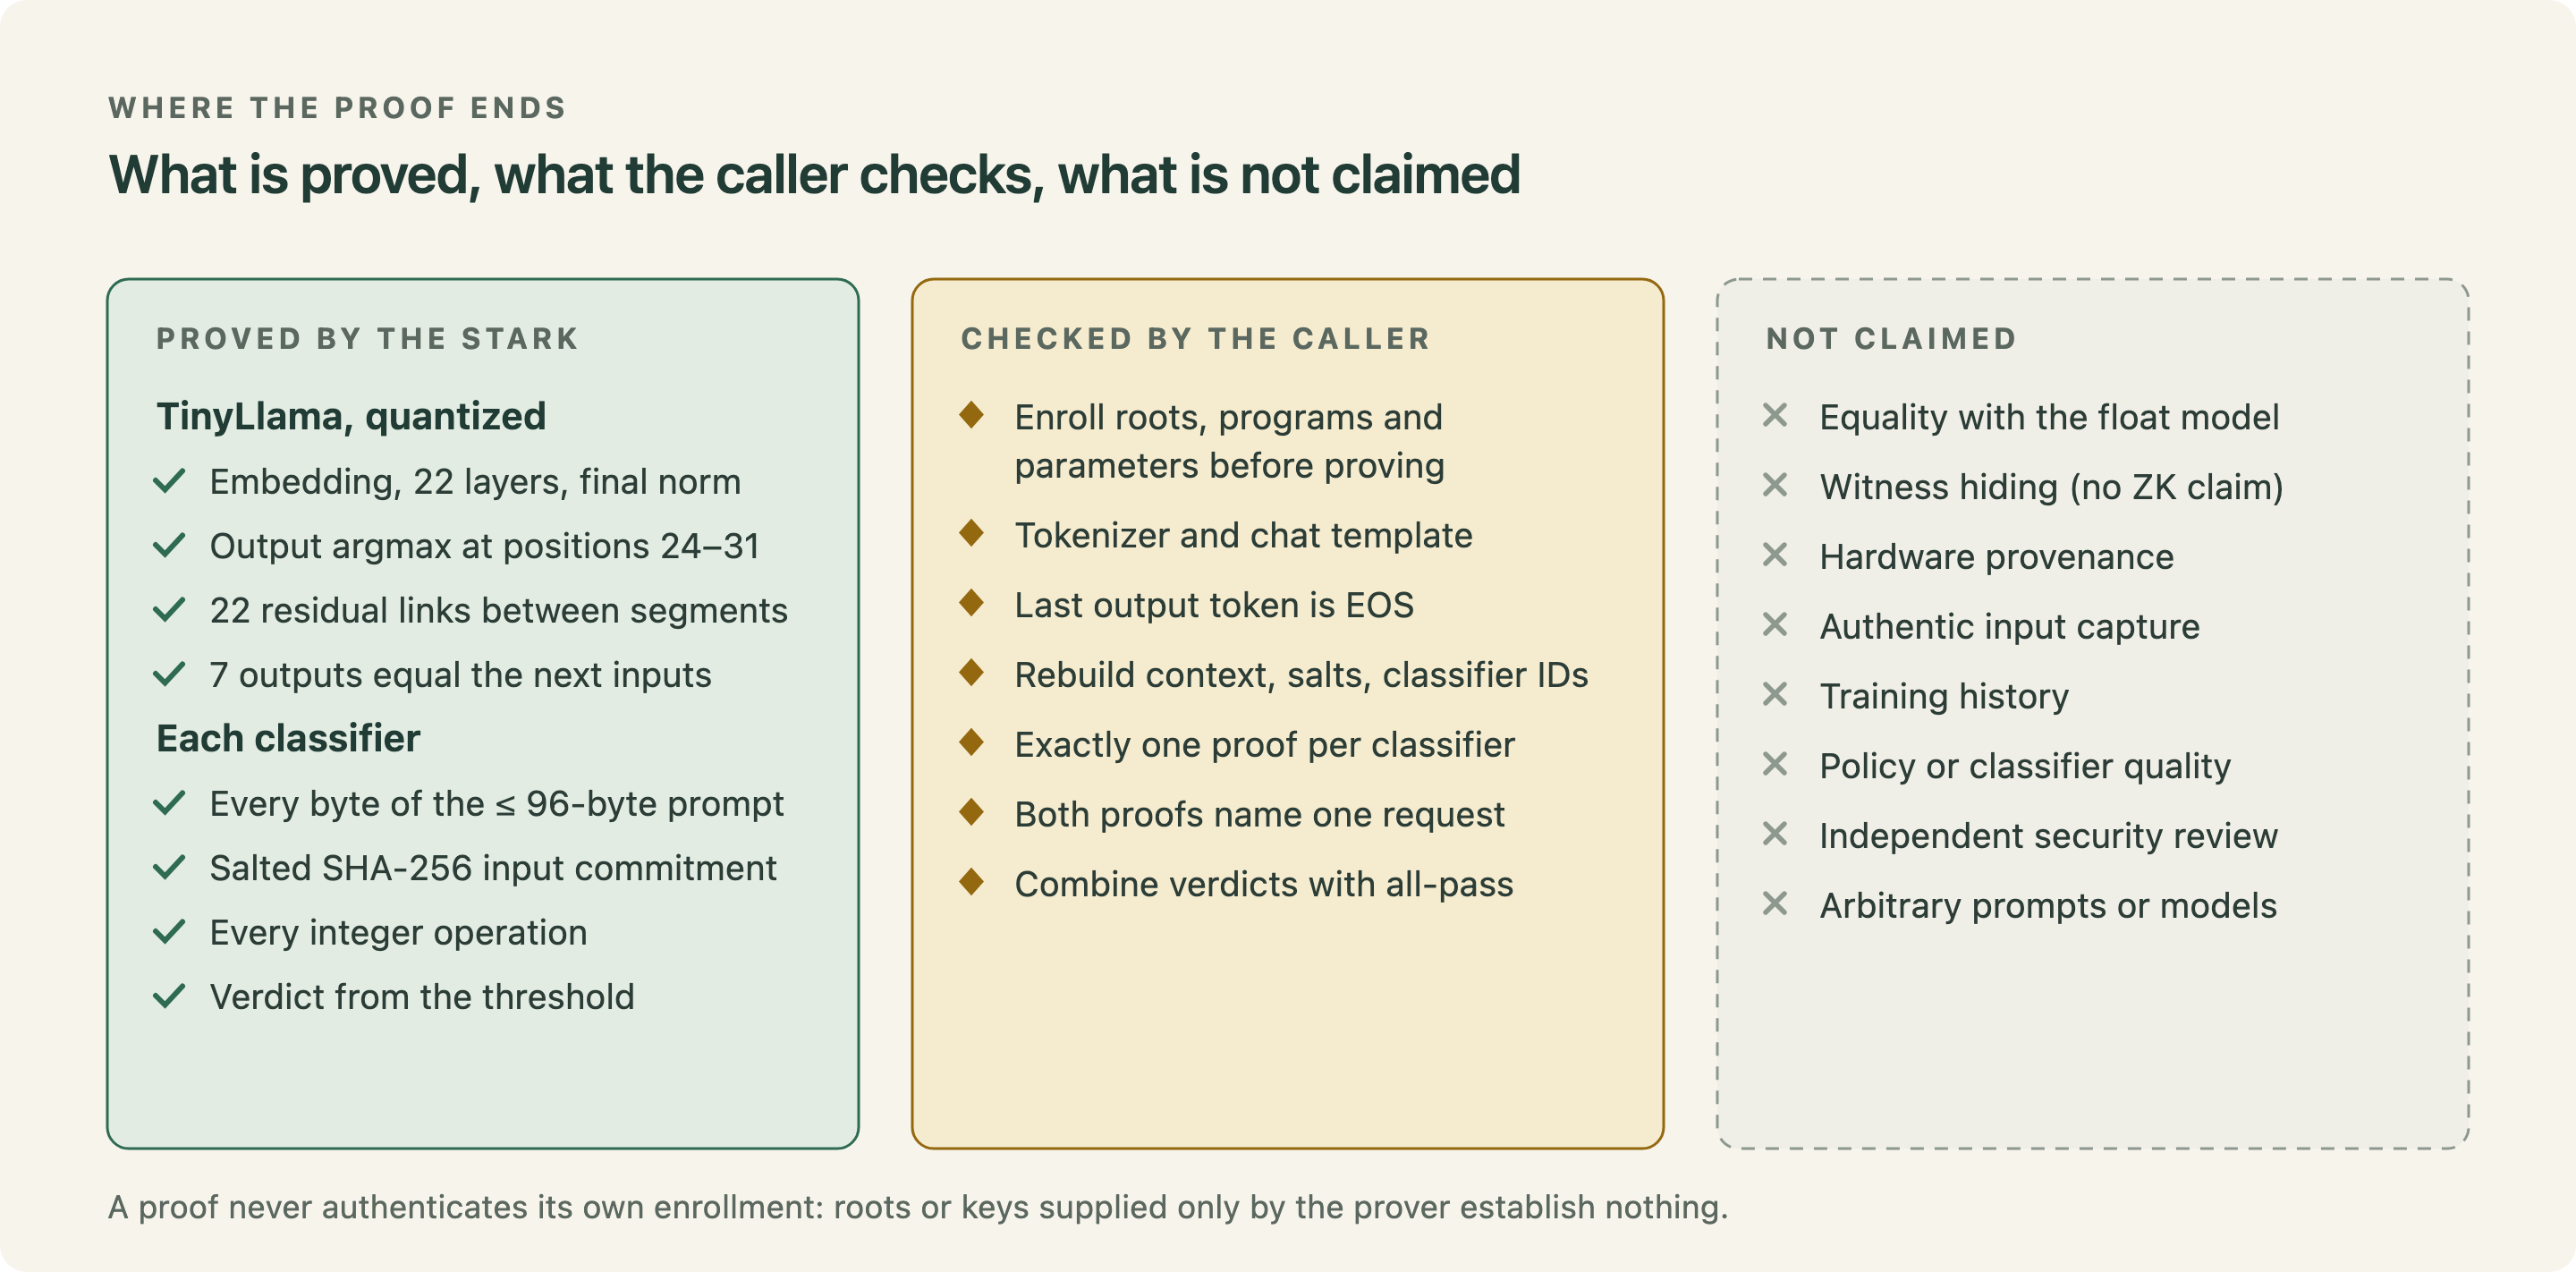
\includegraphics[width=\linewidth]{trust-boundary.png}
\caption{\emph{Where the proof ends.} Three columns: what the STARKs prove, what the caller checks, and what is not claimed. Source: \texttt{docs/\allowbreak{}assets/\allowbreak{}figures/\allowbreak{}trust-\allowbreak{}boundary.\allowbreak{}svg} in the Hallmark repository.}
\label{fig:boundary}
\end{figure}


\subsection{Proof parameters and conjectured soundness}

Table 3 lists the proof parameters as recorded. Both configurations use Blake2s-based Merkle commitments and transcripts.

\textbf{Table 3.} Concrete proof parameters and the figure given by the library formula. The last row is a query-and-grinding conjecture, not a proven or qualified security level (Section 5.3).

{\small
\begin{xltabular}{\linewidth}{XXX}
\toprule
\textbf{Parameter} & \textbf{SASH prover (LLM segments)} & \textbf{Direct S-two classifiers} \\ \midrule
\endhead
FRI queries & 100 & 80 \\
Log blowup factor & 1 & 4 \\
Last-layer log degree bound & 0 & 5 \\
Proof-of-work bits & 0 & 16 \\
Fold step & 1 & 1 \\
Formula: proof-of-work bits + log blowup × queries & 100 & 336 \\
\bottomrule
\end{xltabular}}

The formula is the one the S-two library itself computes. In version 2.2.0, the exact version Hallmark pins, it returns the proof-of-work bits plus the log blowup factor times the number of queries (source locations in Appendix A) \cite{A28}. The same query-and-grinding form is the first of three values whose minimum StarkWare's earlier ethSTARK prover reports as its ``conjectured security'', and the prover's repository points separately to a proven bound on FRI soundness \cite{A39}, \cite{A40}; the ethSTARK documentation describes the statement that prover proves \cite{A43}. We attribute the conjecture to the repository, whose text we read, because we could not retrieve the documentation to check its wording. For the classifiers the formula gives 16 + 4 × 80 = 336, a query-and-grinding conjecture that the unanalysed extension-field and hash terms below cap, not a proven bound. Applied to each LLM segment's parameters it gives 0 + 1 × 100 = 100, which matches the 100 conjectured bits that the SASH prover reports for its configuration \cite{SASH}; the Hallmark repository records that this is not an independent security qualification.

Three qualifications apply. First, the formula counts only query and grinding terms and rests on the conjectures of Section 4.3; it is not a proven bound. For orientation only, counting the query term of the proven analyses (plus the classifiers' 16 proof-of-work bits), the unique-decoding regime gives about 41.5 bits per LLM segment (100 × −log₂ 0.75, at rate 1/2) and about 89 for the classifiers (16 + 80 × −log₂ 0.53125, at rate 1/16), and the regime up to the Johnson bound \cite{A40} gives at most about 50 and 176. These approximations are our own; they ignore the commit-phase and field-size terms, which can only lower them, and they are not a provable bound for either configuration. Second, every figure above ignores other limits, among them the secure extension field QM31 (degree 4 over Mersenne-31, about \ensuremath{2^{124}} elements) and the hash's collision resistance, which cap both configurations, so the classifier configuration reaches less than the conjectured 336. Third, the LLM evidence composes 23 proofs. By a union bound, the bundle's conjectured soundness error is at most 23 times the per-proof error, which loses at most log₂ 23 ≈ 4.52 bits, about 95.5 conjectured bits for the bundle. This is our own derivation, not a statement of any source. Formal verification of an S-two AIR does not extend to Hallmark's classifier or LLM AIRs \cite{A30}. Hallmark's class-5 placement is therefore that of a class-5 relation at unqualified parameters, and the dashed edges of Figure 1 need not hold for it: they hold only under the reading that counts proof soundness within K.

\subsection{What the case illustrates}

We read the recorded experiments against four points. The first, second and fourth follow from the definitions of Section 4 once Hallmark's relations are fixed, so the case shows them concretely rather than testing them; the third concerns cost, which only matched measurement could settle.

\textbf{Residual trust sits in enrollment and host reconstruction.} \emph{Skip} fails if the verifier requires the complete roster of proofs before it accepts the answer; a verifier that asks for proofs only later turns Skip into Defer. \emph{Swap} fails because classifier identity, program hash and threshold are fixed by enrollment. \emph{Substitute} fails at the enrolled model, shape and calibration roots. \emph{Replay} fails because the input commitment and context digest are public inputs the caller recomputes (Section 5.2). \emph{Misreport} fails because the circuit constrains the public verdict to the threshold decision. Each defence holds only under the caller's enrollment and reconstruction, which are E and P. None addresses capture provenance: if the operator chooses R, every proof can be valid for a request the user never sent.

\textbf{For exact integer relations with public weights, replay needs less trust than a proof.} The classifier weights and witnesses are public, and the demonstration's caller already reruns native inference to derive the expected verdicts; replay of an exact integer program needs only \{E, P\}, while the proof needs \{E, P, K\} at unqualified parameters. In the demonstrated configuration the classifier proofs therefore add no integrity evidence for this caller. The same holds for a verifier that holds the TinyLlama weights, since a rerun under the proved relation reproduced the proved answer (exp-R1-native-rerun). The proofs become non-redundant only for a verifier that lacks the weights or will not re-execute; a deployment with private weights would also need hiding, which Hallmark lacks (Box 1).

\textbf{Proofs remove the verifier's need for weights and re-execution; the timings settle nothing about time.} The proofs let a verifier check the answer without the TinyLlama checkpoint (about 2.2 GB) and without executing any model, at the price of obtaining a 737,858,641-byte bundle. Whether this is also faster than a rerun is not settled by the records, and we make no claim either way. The recorded figures (Table 4) are 3.40--3.53 s to verify the 23-proof LLM bundle, against medians of 0.769 s for one quantized greedy answer under the proved relation and 0.235 s for an fp32 reference answer; and 0.807 s for nine proof-only classifier verifier processes, against about 0.61 s for the nine native executions. They support no direction, for three reasons. All of these ran on the same Apple M4 Max. The boundaries differ in both directions: verification timers include process start and proof loading, while the LLM rerun timers exclude model loading, calibration and tokenization; and the 3.40--3.53 s verifier path has the model roots compiled in, which spares it the runtime root derivation (Section 5.5). The classifier verification total rests on one cold first process, 0.345 s of 0.807 s against 0.050--0.079 s for each of the other eight; that process alone takes more than four times as long as any other, so one cold start sets the sum. And the CNN rerun, about 0.2 s per request and nearly all of the 0.61 s, times Hallmark's pure-Python reference interpreter, whose timed call also hashes the weights and tokenizer, validates the input profile and decodes the program constants before it evaluates the integer graph; it measures that implementation, not the integer program. A comparison would need warm, repeated verifier runs, a compiled rerun with loading and hashing outside the timer, and matched boundaries for the LLM; none was run. Hallmark instantiates the trust set of class 5, not a cost profile.

\textbf{Evidence for S cannot show gating or timing.} The artifact exhibits both gaps. The CNN's verified verdict on the France prompt is block, a verified proof of an answer to that prompt exists, and the composed result reports that the request does not pass. Nothing in the evidence shows whether that answer was withheld. The three classifier proofs were produced on 2026-10-28, two days after the answer proofs they were joined with, and the caller accepted the join (exp-L1-llm-proving, exp-J1-composition). For this statement, proving after the fact cannot be told apart from proving in line.

\subsection{Recorded costs and rejection evidence}

The case reads six experiments. Five ran on the Hallmark repository between 2026-10-26 and 2026-10-29, before this analysis: \textbf{exp-L1-llm-proving} (the 23 segment proofs as one CPU/CUDA matched pair on one NVIDIA H200 via Hugging Face Jobs, plus native verifier checks on the Mac); \textbf{exp-C1-classifier-proving} (one instrumented run on an Apple M4 Max with 16 CPU cores, 48 GiB and 4 prover threads that trained the classifiers and produced and verified nine proofs, three classifiers × three requests); \textbf{exp-A100-classifier-cuda} (the nine C1 prover commands, CPU against CUDA, as three matched pairs on an A100-SXM4-80GB); \textbf{exp-J1-composition} (host composition of the L1 proofs with three new classifier proofs on the same request); and \textbf{exp-V1-rejection-validation} (mutation and conformance runs on main commit \texttt{1bc6b72}). The sixth, \textbf{exp-R1-native-rerun}, was run for this revision on the same M4 Max (macOS 26.6.2, 2026-10-30): 50 timed executions per classifier and request, and five timed LLM answers per variant. The costs are recorded single-run figures, two repeat checks, medians of three matched pairs, or, for exp-R1, medians with ranges. We quote no ratio between quantities measured on different machines.

\textbf{Table 4.} Recorded costs with timer boundaries.

{\small
\begin{xltabular}{\linewidth}{XXXX}
\toprule
\textbf{Quantity} & \textbf{Value} & \textbf{Boundary} & \textbf{Experiment} \\ \midrule
\endhead
LLM proving, CUDA & 53.94 s & SASH sessions summed over 23 segments; complete GPU commands 155.89 s & exp-L1-llm-proving \\
LLM proving, CPU SIMD & 547.75 s & Same sessions on CPU, same host; complete commands 679.49 s & exp-L1-llm-proving \\
LLM verification, Mac & 3.53 s and 3.40 s & One full-bundle check each; native verifier with roots compiled in; thread configuration not recorded & exp-L1-llm-proving \\
LLM verification, Linux & 77.40 s and 77.61 s & One full-bundle check each; fresh verifier deriving roots at runtime & exp-L1-llm-proving \\
LLM proof bundle & 737,858,641 B & 23 JSON files; excludes enrollment, keys, statements & exp-L1-llm-proving \\
LLM native rerun, quantized & median 0.769 s (0.752--0.822; n = 5) & One greedy answer through EOS, CPU, 4 threads; excludes model load, calibration, tokenization & exp-R1-native-rerun \\
LLM native rerun, fp32 & median 0.235 s (0.234--0.236; n = 5) & Same boundary; Transformers greedy generation & exp-R1-native-rerun \\
Classifier proving & 24.06 s & Nine final S-two proving calls; complete prover commands 50.03 s & exp-C1-classifier-proving \\
Classifier verification & 0.807 s (first, cold process 0.345 s; the other eight 0.050--0.079 s) & Nine fresh proof-only verifier processes, run once each; each includes process start and proof loading; thread configuration not recorded & exp-C1-classifier-proving \\
Classifier native rerun & medians 0.274--0.284 ms (rule), 0.979--0.991 ms (MLP), 199.9--203.8 ms (CNN); n = 50 each & One in-process call of the pure-Python reference interpreter, after warm-up; for the CNN the call includes hashing of weights and tokenizer, validation and constant decoding; excludes artifact loading, export, witness construction; one thread & exp-R1-native-rerun \\
Classifier proofs & 18,063,779 B & Nine files of 1.93--2.15 MB; excludes enrollment, keys & exp-C1-classifier-proving \\
Classifier prover commands, A100 & 92.41 s → 22.22 s & CPU → CUDA; median of three matched pairs of nine commands & exp-A100-classifier-cuda \\
Composed command & 266.29 s & Native LLM workflow (build, two honest checks, 36 mutations), three new classifier proofs and the join & exp-J1-composition \\
\bottomrule
\end{xltabular}}

The 53.94 s LLM figure counts proving sessions only, and its timer also includes interaction work. The two LLM verifier paths differ in platform and in root handling, which the record cannot separate, and runtime root derivation was not timed separately (Section 7.2); runtime root derivation may not be succinct, and compiling the roots in moves them into enrollment, so on the 3.40--3.53 s path they belong to E (exp-L1-llm-proving). The exp-R1 reruns reproduced the published verdicts, and both LLM variants returned the proved answer token identifiers: for this one prompt the fp32 greedy answer equals the proved quantized answer, a single case rather than an agreement rate. The exp-R1 records carry the platform, core count and thread settings but not the code commit or the CPU model; they were produced on the Apple M4 Max named above from the repository at commit \texttt{adddf9a} with the measuring script added, and the script now records both fields. The classifier exports they read are fixed by the loader, which accepts only the published quantizations (SHA-256 \texttt{f8090161\allowbreak{}455ee56c\allowbreak{}dcd73eaa\allowbreak{}b44437ef\allowbreak{}a3b278a7\allowbreak{}86d7c246\allowbreak{}491da5f1\allowbreak{}e1431a9c} for the MLP and \texttt{8de31ae0\allowbreak{}215178f5\allowbreak{}c74aa43e\allowbreak{}58dd6351\allowbreak{}1bc3b6a8\allowbreak{}81c2045c\allowbreak{}c96def9e\allowbreak{}149b8f0b} for the CNN; \texttt{scripts/\allowbreak{}run\_e2e.\allowbreak{}py}); a fresh \texttt{make e2e} on 2026-11-02 retrained both and reproduced these digests.

All recorded engineered mutations were rejected: 122 tampering cases across the classifier and LLM checks, 16 named join-level mutations and 22 invalid-witness cases. Appendix A lists them, with what they do and do not test, and the memory and run-history notes.

\subsection{Placement}

Table 5 is the single statement of where the instance sits; Box 1 lists what it does not claim.

\textbf{Table 5.} Hallmark placed in the systematization.

{\small
\begin{xltabular}{\linewidth}{XXX}
\toprule
\textbf{Class or property} & \textbf{Status} & \textbf{Basis} \\ \midrule
\endhead
Class 5, classifier integrity & Class-5 relation at unqualified parameters & Verdict = 1 iff F(x) < t on a committed prompt ≤ 96 bytes; nine proofs verified (exp-C1-classifier-proving); formula figure 336, a conjecture, not a proven bound (§5.3) \\
Class 5, LLM integrity & Class-5 relation at unqualified parameters, as a linked bundle & 23 segments, 22 residual links, 7 token links (exp-L1-llm-proving); about 95.5 conjectured bits for the bundle by our union bound (§5.3) \\
Residual P & Self-verified LLM bundle; host links and join & No independent LLM verifier (§5.1) \\
Request binding & Within each relation by proof; across relations by host check & 18 cross-request rejections (exp-V1-rejection-validation); 16 join-level rejections (exp-J1-composition) \\
Class 1, replay & Gives the same classifier integrity with less trust in the demonstration & Caller reruns native inference; exact integer relations (§5.4) \\
Cost profile of class 5 & Not established & Not compared with a rerun (§5.4; exp-R1-native-rerun, exp-C1-classifier-proving) \\
Classes 2 and 4 & Not reached & No per-request record (gap 1, §7.1); no attestation \\
Hiding, capture provenance & Not reached & Box 1 \\
Gating and timing (S′) & Not reached & S has no G or T clause; J1 joined classifier proofs made two days after the answer proofs (§5.4) \\
Adequate safety policy & Not reached & Synthetic classifiers; MLP score bound [−5600, −2338] below threshold 0, so it never blocks; the CNN blocks the demonstration prompt \\
\bottomrule
\end{xltabular}}

\section{Related Work}

\textbf{Proofs of ML inference.} Verifiable neural-network inference began with interactive proofs for small networks \cite{A1} and moved to SNARKs for CNNs \cite{A5} and ImageNet-scale models \cite{A7}, with compilers that co-design quantization and proving \cite{A4} or optimize circuit layout \cite{A8}, or compile models to basic blocks \cite{A13}. LLM provers cover full 13B inference \cite{A15}, all generated tokens of GPT-2 and Gemma 3 \cite{A17}, agent transcripts with tool outputs \cite{A19}, and sampled layerwise coverage up to 70B with prompt and answer binding \cite{A22}. Jolt Atlas applies lookup arguments to Open Neural Network Exchange graphs \cite{A14}, and ML has been compiled to S-two before \cite{A29}. Hallmark contributes no proof system.

\textbf{Attestation-based inference and audits.} Benchmarks of confidential computing report moderate overhead for LLM inference on CPU and GPU TEEs \cite{B8}, \cite{B10}. Cai et al. propose TEEs as a practical remedy for model substitution in APIs \cite{C15}. Attestable Audits runs safety benchmarks in Nitro enclaves and binds prompt and response in an interaction attestation \cite{B23}. Proof-of-Guardrail asks our question and answers it with an attested wrapper whose classifier call leaves the measured boundary (Section 4.3) \cite{B24}. Deployed services already compose attestation with transparency: in Apple's Private Cloud Compute, user devices send data only to nodes that cryptographically attest to running publicly listed software, and the log and binary images are made publicly available for inspection \cite{B26}, a class-4 and class-2 composition at production scale, built for privacy rather than for guardrail verdicts. Cove composes TEE-attested computations into multi-party audit workflows, including attested inference \cite{B25}.

\textbf{Safety and fairness claims with proofs.} South et al. produce zkSNARK attestations that a private-weight model meets aggregate accuracy, bias or safety metrics on a dataset \cite{A9}. ZkAudit proves that published commitments to data and weights derive from training \cite{D19}. FairProof issues a fairness certificate specific to each user query, under a model kept confidential through commitments and zero-knowledge proofs \cite{F3}. It is precedent for per-input proofs of a safety-relevant property, though not of a guardrail verdict. A vendor blog describes wrapping an automated-reasoning guardrail pipeline in zkML so that ``every action carries cryptographic proof of execution'', without a binding mechanism or a published evaluation \cite{E1}.

\textbf{Replay, delegation and logs.} Refereed delegation goes back to protocols in which several servers compute and a referee resolves disagreement cheaply \cite{C6}, \cite{C7}; Arbitrum \cite{C8}, opML \cite{C9} and Verde \cite{C10} carried challenge-and-bisect to smart contracts and ML. Zhou binds agent tool use with signatures and shows that replay-based verification yields only a probabilistic bound \cite{A38}. Keyless signing gives identity-bound records \cite{C20}, and model signing applies it to weights \cite{C22}.

\textbf{Accountability and audit.} Kroll et al. argue that automated decisions can be made accountable by assuring procedural regularity, meaning that decisions follow an announced set of rules, verifiable without revealing key attributes of the decisions \cite{F5}. Enrollment before proving is a concrete instance of rules announced in advance. Internal audit frameworks address the accountability gap through documented internal process \cite{D15}; the evidence systematized here is instead checkable from outside the organisation, request by request. It sits at the application layer of a layered audit \cite{D16}, where it adds evidence that black-box access cannot provide \cite{D18} without replacing governance or model audits.

\textbf{Orderings of evidence.} Peng et al. and Xia et al. order evidence classes by verifiability \cite{A32}, \cite{A35}. RAILS, a clearing design for agentic commerce, orders its admissibility classes as SELF ⪯ SIGN ⪯ \{WIT, REC\} ⪯ ATT ⪯ PROOF and states that they ``form a partial order, not a scalar ranking'' \cite{F9}. RAILS's witness and receipt classes have no single counterpart in ours, so we compare SELF, SIGN, ATT and PROOF, where the two orders differ in two places. RAILS places signed records above self-report; for the integrity of a verdict ours merges them, because a signature by the operator authenticates the record, not the computation (Section 4.3). And RAILS places proofs above attestation without qualification, whereas ours makes that edge conditional on counting proof-system soundness at the deployed parameters within K, and drops it for proofs that need a setup ceremony. RAILS has no replay, statistical or refereed classes, and its relations are asserted class by class; ours are readings of explicit trust sets, so a reader can see which assignment each edge depends on, and ours also records request binding, capture provenance, gating and timing per class. Rizzini et al. systematize integrity claims in privacy-preserving federated learning, binding each claim to a round identifier against replay, but do not order mechanisms \cite{F7}. Formal verification of guardrail classifiers addresses adequacy, the axis our order leaves out \cite{E2}.

\textbf{Search outcome and novelty.} The earlier version of this paper bounded its novelty statement by three works screened at abstract level; we have now read them. Balan et al. propose cryptographic verifiability for an AI pipeline from data to inference and unlearning; they prove inference on a given input, but bind no request, treat no guardrail and compare only TEEs with proofs \cite{F6}. Rizzini et al. \cite{F7} concern federated learning, not LLMs or guardrails. Ker\v{s}i\v{c} et al. survey and compare on-chain zkML frameworks \cite{F8}; we could read only the abstract, which does not concern guardrails. The guardrail companion work named in the Jolt Atlas paper, which claims zkML for ``succinctly verifiable agentic guardrails'' \cite{A14}, was searched for on arXiv, the IACR archive and the authors' site, and not located. That site lists a forthcoming work, with a preprint available on request, on verifiable receipts that a policy check was enforced on an agent action \cite{F10}; we have not read it. With the vendor blog \cite{E1}, these are the closest same-question works on the proof side; they concern automated-reasoning policy checks, not classifiers. To our knowledge, based on the searches described in Section 3 and completed on 2026-10-30, no peer-reviewed or preprint work reports succinct per-request proofs of a guardrail-classifier verdict composed with an LLM-answer proof. The statement is narrow: each element of the case has precedent (Sections 4 and 6), the classifiers are synthetic and the composition is a host join. The case matters here for what it shows about the order, not for priority.

Table 6 gives published figures for orientation only, and marks a setup ceremony (N) only for Seal-then-sample, the one system whose setup we checked; models, statements, hardware, coverage and timer boundaries all differ, so no ranking is implied. Table 7 positions the case against the closest works.

\textbf{Table 6.} Published figures from other systems. Every row is \textbf{not matched} to Hallmark or to any other row.

{\small
\begin{xltabular}{\linewidth}{XXXX}
\toprule
\textbf{System} & \textbf{Class} & \textbf{Reported figure} & \textbf{Conditions as reported} \\ \midrule
\endhead
zkCNN \cite{A5} & 5 & 88.3 s prove; 341 KB; 59.3 ms verify & VGG16, 15M parameters; hardware not given in the abstract \\
zkLLM \cite{A15} & 5 & Under 15 min prove; under 200 kB proof & 13B model, full inference; one NVIDIA A100 40 GB GPU; 2048-token input \\
DeepProve repository \cite{A18} & 5 & 7.6 min / 19 min prove; 1.3 s / 4.3 s verify & GPT-2 / Gemma 3; 512-token sequences; 24-core CPU, 504 GB RAM \\
zkAgent \cite{A19} & 5 & 93.18 s prove; 1.63 s verify & One coding-assistant transcript; hardware not given in the abstract \\
Seal-then-sample \cite{A22} & 5 + 3a; needs N & 1,259 s prove; 4.34 MiB; 46.3 s verify & Llama-2-70B, 5 of 163 chunks proved; 2 TB CPU host; HyperKZG with a test reference string \\
Proof-of-Guardrail \cite{B24} & 4 (wrapper) & About 5.1 ms verify; about 97.8 ms attestation generation & AWS Nitro enclave (m5.xlarge) running a guardrail wrapper; Llama Guard 3-8B via the OpenRouter API, outside the measurement \\
\bottomrule
\end{xltabular}}

\textbf{Table 7.} Positioning against the closest works. The Proof-of-Guardrail placement depends on modelling its external classifier API as operator-reliant (Section 4.3), and its row concerns a real 8B guardrail where Hallmark's classifiers are synthetic.

{\small
\begin{xltabular}{\linewidth}{XXXXX}
\toprule
\textbf{Work} & \textbf{Class} & \textbf{Same question?} & \textbf{What it provides that Hallmark does not} & \textbf{What Hallmark provides that it does not} \\ \midrule
\endhead
Proof-of-Guardrail \cite{B24} & 4 for the wrapper; classifier computed by an external API & Yes & A real guardrail classifier; millisecond verification; a serve-time report whose measured wrapper can cover gating and timing & The verdict computed inside a proved relation, with no attestation root, at the price of proof soundness at unqualified parameters; a joined answer proof \\
Seal-then-sample \cite{A22} & 5 + 3a; needs N & LLM half only & Prompt and answer binding inside one LLM proof; scale to 70B & A classifier-verdict proof joined by host check to a full-coverage answer bundle produced by the SASH prover \\
FairProof \cite{F3} & 5 & Partly (per-query fairness) & Confidential model; per-query fairness certificate & A threshold-classifier verdict joined to an answer proof \\
Attestable Audits \cite{B23} & 4 & Partly (benchmarks) & Confidential model and data; Llama-3.1-8B benchmark runs & Proof soundness in place of an attestation root; per-request classifier verdict \\
\bottomrule
\end{xltabular}}

\section{Toward an Auditor-Ready Receipt, and Limitations}

\subsection{Gaps}

A receipt a deployer could hand to an auditor would need more than any single class provides. We list the gaps by the property each concerns, with the compositions in the literature that could supply it. None is estimated here, apart from the order of magnitude of proving cost in gap 4.

\begin{enumerate}
\item \textbf{Gating and timing (S′).} Evidence for S is consistent with an operator that ignores a block verdict or proves after serving (Section 5.4). Two compositions could reach S′. An attested wrapper that withholds the answer on a block verdict and reports at serve time covers G and T \cite{B24}; composed with a proof whose public input is the wrapper's request commitment, it would also move the verdict computation inside a proved relation. A logged record of the proofs' public inputs, written before the answer is released, would fix the claimed verdict in time for later proofs to match \cite{C16}, \cite{C18}, though it would not show that the classifier ran in line. Deployed attested services \cite{B26} and attested audit workflows \cite{B25} show that the attestation half has been built at production scale \cite{B26} and composed into audit workflows \cite{B25}; in our sources neither reports gating on a classifier verdict. Neither composition is shown here.
\item \textbf{Capture provenance.} The proofs bind a committed prompt, not the prompt a user sent. DECO lets a user prove that data accessed over TLS came from a particular website, without trusted hardware or server-side changes \cite{F4}, which makes it a primary route for authenticated capture; zkAgent applies such sub-proofs to agent transcripts \cite{A19}. Interaction attestations \cite{B23} and pre-committed per-request logs \cite{C13} are alternatives, and an attested capture service could write the request commitment into its report data \cite{B2}.
\item \textbf{Hiding.} With public witnesses, a deployer cannot hand auditors prompts containing user data without a separate privacy basis. Weight privacy is costly in other stacks (Mystique reports 28 min for ResNet-101 with a committed private model against 5 min with a public one \cite{A6}), and no source we hold measures it on a Circle STARK stack. Public witnesses let the auditor read the committed classifier, which blunts the hidden-weight attack \cite{A23}; a hiding variant would need another way to give that assurance.
\item \textbf{A verifier cheaper than a rerun.} The recorded case does not establish one (Section 5.4). Proving is a separate cost: the 1.1B answer took about 54 s of proving sessions, 156 s as complete GPU commands, on one H200 (Table 4), so proving in line, before release, would add about one to three minutes per request for this model on that hardware.
\item \textbf{Enrollment governance.} The case moves residual trust to enrollment (Section 5.4), and no class supplies it. Someone must fix the reference classifiers, thresholds, model roots and fallback policies, and evidence when each was fixed or changed, before the requests it governs. In RATS terms this is the Reference Value Provider's role \cite{B5}; model signing \cite{C22} and transparency logs \cite{C18} could record enrollment and threshold changes before use. Who should enroll (the deployer, an auditor or a regulator) is left open; the choice decides whom E asks the verifier to trust.
\item \textbf{Real guardrails.} The smallest real guardrail classifier in our sources, Prompt Guard 2, has 22 million parameters and a 512-token context \cite{D6}, and open guardrails reach a 12-billion-parameter multimodal classifier \cite{D4}; no source we hold proves one at class 5. Since the proved LLM relation has 1.1 billion parameters, size alone does not rule out the former, but its context, architecture and integer-export fidelity would have to be shown.
\item \textbf{Qualification.} A provable soundness bound for both configurations, an independent LLM verifier, formal verification of the gate-level AIRs \cite{A30}, and witness-level testing of the gadgets against the circuit-failure classes of Section 4.3 \cite{F1} are all missing.
\item \textbf{A compact receipt.} The LLM evidence is a 737,858,641-byte linked bundle per request and the join is host code. Under the AI Act, providers of high-risk AI systems must keep the logs their systems automatically generate, to the extent the logs are under their control, for a period appropriate to the system's intended purpose and of at least six months unless Union or national law provides otherwise (Art. 19(1)) \cite{C26}, and deployers have the same duty (Art. 26(6)) \cite{C26}. We do not argue that a guardrailed chat service is high-risk, and the Act, as read, does not ask that logs be proofs, so we claim no retention cost; retaining one bundle of this size per request would simply scale with request volume. A deployer need not prove every request: committing every request's public inputs to a log before release, and proving or verifying only a sample or on challenge, is the pattern IMMACULATE uses \cite{C13}. It also constrains Defer, since an operator that commits to a verdict before computing it is caught whenever a sampled proof disagrees.
\item \textbf{Multi-rail and output pipelines.} Guardrail frameworks orchestrate several rails \cite{D7}, \cite{D11}; Hallmark proves individual input classifiers combined with \texttt{all-\allowbreak{}pass}. No source we hold treats proofs over rail orchestration logic, output rails under streaming release (Section 2.2) or fail-open fallbacks (Section 2.3).
\item \textbf{Record keeping over time.} The AI Act requires high-risk AI systems to allow automatic recording of events (Art. 12(1)) \cite{C26}, and the Code of Practice asks providers of general-purpose AI models with systemic risk to implement and document mitigations such as input and output filtering (Measure 5.1, Safety and Security chapter as published on 10 July 2025) \cite{D24}. Neither text, as read, mandates cryptographic per-request evidence, so the systematization offers possible forms of evidence rather than meeting a stated demand; we read the Regulation as published in the Official Journal of 12 July 2024 and have not verified whether later amendments change these articles. Transparency logs are a deployed template for such records \cite{C18}, and Hallmark records none.
\end{enumerate}

\subsection{Limitations}

The study has six limitations. First, the case is one instance: one prompt, one model profile and classifier inputs of at most 96 bytes, so what it shows is illustration, not a test or a measurement of generality. Second, the experiments were run by the author, who also built the artifact, and the trust universe was drawn with the results known; Section 4.2 states which edges depend on its granularity. Third, reading depth varies across sources (Section 3). Fourth, the validation mutations are engineered test cases, not an adversarial evaluation: there is no witness-level fuzzing and no completeness argument for the gadgets (Appendix A), and the LLM verifier is the prover's own implementation (Section 5.1). Fifth, the code, the research record and this manuscript were produced with AI assistance (back matter). Sixth, two questions are left open: runtime root derivation was not timed separately from LLM verification (Section 5.5), and the relation, if any, between Seal-then-sample \cite{A22} and the SASH prover was not established, so we assert none (Section 5.1). The order also concerns one statement, S. A different statement, such as model-level safety metrics \cite{A9} or training provenance \cite{D19}, may order the same mechanisms differently.

\section{Conclusion}

Evidence that a safety classifier ran on a request is not one thing. Each class establishes something different and asks the verifier to trust something different. Written as trust sets, most pairs of classes above the operator-reliant bottom cannot be ranked, and proofs sit above attestation only if proof soundness at the deployed parameters is folded into the cryptographic assumptions other classes need, and only for proofs without a setup ceremony. Every compared class speaks to what was computed. Gating and timing, the senses of ``ran'' an auditor often cares about most, need a mechanism on the serving path, which some attestation and logging designs can provide and a proof of S cannot. In the Hallmark case, residual trust sits in the caller's enrollment and host checks; for its exact integer classifiers with public weights, replay needs less trust than the proofs; its proofs spare the verifier the weights and the re-execution; and its own composition accepted proofs made two days after the answer. The next steps are compositions that reach S′ (an attested, gating wrapper or a pre-release log composed with proofs), authenticated capture, governed enrollment, a provable soundness bound, and a proof of a real guardrail classifier.

\section*{Data and Artifact Availability}

The Hallmark code is public under the MIT licence at \url{https://github.com/AbdelStark/hallmark}. The proofs, logs and machine records behind the figures of exp-L1, exp-C1, exp-A100, exp-J1 and exp-V1 are published as the GitHub release \texttt{circle-\allowbreak{}reference-\allowbreak{}2026-\allowbreak{}10-\allowbreak{}28} (\url{https://github.com/AbdelStark/hallmark/releases/tag/circle-reference-2026-10-28}); \texttt{docs/\allowbreak{}REFERENCE-\allowbreak{}RUN.\allowbreak{}md} explains how to download and verify them. The trained classifiers are published on Hugging Face as \texttt{abdelstark/\allowbreak{}hallmark-\allowbreak{}byte-\allowbreak{}mlp} and \texttt{abdelstark/\allowbreak{}hallmark-\allowbreak{}contextual-\allowbreak{}byte-\allowbreak{}cnn}. The experiments map to frozen records under \texttt{research/\allowbreak{}evidence/\allowbreak{}}: exp-L1-llm-proving, exp-C1-classifier-proving and exp-J1-composition to \texttt{circle-\allowbreak{}reference-\allowbreak{}2026-\allowbreak{}10-\allowbreak{}28.\allowbreak{}json} and \texttt{llm-\allowbreak{}gpu-\allowbreak{}generated-\allowbreak{}constraints-\allowbreak{}2026-\allowbreak{}10-\allowbreak{}26.\allowbreak{}json}, with the L1 bundle size in \texttt{llm-\allowbreak{}gpu-\allowbreak{}benchmark-\allowbreak{}2026-\allowbreak{}10-\allowbreak{}26.\allowbreak{}json} and the J1 retained-composition materials in \texttt{circle-\allowbreak{}default-\allowbreak{}2026-\allowbreak{}10-\allowbreak{}28.\allowbreak{}json}; exp-A100-classifier-cuda to \texttt{classifier-\allowbreak{}gpu-\allowbreak{}benchmark-\allowbreak{}2026-\allowbreak{}10-\allowbreak{}28.\allowbreak{}json}; exp-V1-rejection-validation to \texttt{audit-\allowbreak{}fixes-\allowbreak{}validation-\allowbreak{}2026-\allowbreak{}10-\allowbreak{}29.\allowbreak{}json} (main commit \texttt{1bc6b72}); the MLP score bound to \texttt{mlp-\allowbreak{}domain-\allowbreak{}bound-\allowbreak{}2026-\allowbreak{}10-\allowbreak{}27.\allowbreak{}json}. The mutation lists of Appendix A are defined in \texttt{scripts/\allowbreak{}check\_\allowbreak{}circle\_\allowbreak{}composed.\allowbreak{}py} and \texttt{scripts/\allowbreak{}check\_\allowbreak{}circle\_\allowbreak{}classifiers.\allowbreak{}py}. The exp-R1-native-rerun records and the script that produced them are in the repository at \texttt{research/\allowbreak{}evidence/\allowbreak{}native-\allowbreak{}rerun-\allowbreak{}classifiers-\allowbreak{}2026-\allowbreak{}10-\allowbreak{}30.\allowbreak{}json}, \texttt{research/\allowbreak{}evidence/\allowbreak{}native-\allowbreak{}rerun-\allowbreak{}llm-\allowbreak{}2026-\allowbreak{}10-\allowbreak{}30.\allowbreak{}json} and \texttt{research/\allowbreak{}probes/\allowbreak{}native-\allowbreak{}rerun/\allowbreak{}measure\_\allowbreak{}native\_\allowbreak{}rerun.\allowbreak{}py}; they postdate commit \texttt{adddf9a} and entered the repository with this paper (commit \texttt{e71c1e0}). The sources and PDF of this paper are in the repository under \texttt{docs/\allowbreak{}paper/\allowbreak{}}. This analysis reads the repository at commit \texttt{adddf9a}. The proof-system formula of Section 5.3 is read from the \texttt{stwo} crate, version 2.2.0, which Hallmark pins. The LLM prover is the SASH prover, zk-inference-prover from the Singapore AI Safety Hub (\url{https://github.com/sg-ai-safety-hub/zk-inference-prover}), at commit \texttt{eb95bfa8\allowbreak{}87299d16\allowbreak{}37550228\allowbreak{}d42086c2\allowbreak{}7cbb2b3b} (Apache-2.0) \cite{SASH}.

\section*{Ethics Statement}

This study involved no human subjects and no personal data. All prompts are fixed synthetic engineering inputs written for the artifact, and no user requests were collected. The proved classifiers are synthetic and are not offered as a safety policy.

\section*{Author Contributions}

Abdelhamid Bakhta (sole author), following the Contributor Roles Taxonomy (CRediT): Conceptualization, Methodology, Software, Validation, Formal analysis, Investigation, Data curation, Writing -- original draft, Writing -- review \& editing, Visualization.

\section*{Competing Interests}

The author is employed by Lucid Computing and developed Hallmark, a research experiment with a proof-of-concept implementation, as part of that employment. Hallmark is not a Lucid Computing product. The author declares no other competing interests.

\section*{Funding}

This work received no external funding. It was carried out as part of the author's employment at Lucid Computing.

\section*{AI-Use Disclosure}

The Hallmark code and research record were produced with AI assistance, as the project's state record (\texttt{research/\allowbreak{}STATE.\allowbreak{}md} in the public repository) states. This manuscript was drafted and revised by an AI research and writing pipeline that covered literature search, synthesis, outlining, drafting, simulated peer review, integrity checks of citations and numbers against sources, and revision. The author chose the title and the systematization framing, declared the existing experiments, chose to run the native rerun measurement, and chose to withdraw the verify-versus-rerun direction claims after the final simulated review; the other revision and checking decisions were delegated to the pipeline, which also drafted the text and checked it against its sources. The author is responsible for the content. The literature searches used public topic terms only.

\section*{Appendix A: Rejection Evidence}

\textbf{Table A1.} Engineered mutations rejected.

{\small
\begin{xltabular}{\linewidth}{XXX}
\toprule
\textbf{Check} & \textbf{Rejected} & \textbf{Experiment and notes} \\ \midrule
\endhead
Direct public-input mutations (classifiers) & 63 & exp-V1-rejection-validation, \texttt{make e2e}: 9 fresh proofs verified; 253.87 s \\
Cross-request substitutions (classifiers) & 18 & exp-V1-rejection-validation, same run \\
Invalid rosters & 3 & exp-V1-rejection-validation, same run \\
LLM proof mutations & 38 & exp-V1-rejection-validation: 14 baseline, 20 boundary, 2 enrollment, 2 statement; 23 published proofs; 203.59 s \\
Join-level binding mutations & 16 named cases & exp-J1-composition: see text \\
Invalid witnesses & 22 & exp-V1-rejection-validation, conformance command (passed; 3 maximum-input fresh proofs; 187.60 s) \\
\bottomrule
\end{xltabular}}

All recorded mutations were rejected. The first four rows total 122 engineered tampering cases (63 + 18 + 3 + 38). The 18 cross-request rejections test request binding inside the classifier relation, and come from the classifier end-to-end run in exp-V1, not from the composition. The join has its own negative test: the J1 record lists 16 named join-level rejections (\texttt{circle-\allowbreak{}reference-\allowbreak{}2026-\allowbreak{}10-\allowbreak{}28.\allowbreak{}json}, \texttt{.\allowbreak{}metrics.\allowbreak{}composition.\allowbreak{}binding\_\allowbreak{}rejections}). Each case reran the host join with one element changed: four fields of the opened request (prompt, response, system reference, salt); four fields of the expected request (model, nonce, interaction identifier, policy); one public field in each of the three classifier proofs; a missing, duplicated or reordered proof roster; a different request; and a changed caller enrollment (\texttt{scripts/\allowbreak{}check\_\allowbreak{}circle\_\allowbreak{}composed.\allowbreak{}py}).

The 22 invalid-witness cases are counted separately. Each changes one witness value of an honest 96-byte case and checks that proving fails. For each classifier, five values are targeted: a late input byte, a salt byte, an encoded-padding byte, the active-input mask and the verdict. The MLP adds a byte count, a rounded hidden value and the score; the CNN adds the last convolution accumulator, a pooled maximum and a head bit. Twenty-one of these mutations fail at S-two's constraint check. The twenty-second removes a dense coefficient from the CNN program and is rejected by the caller-enrolled program pin (\texttt{scripts/\allowbreak{}check\_\allowbreak{}circle\_\allowbreak{}classifiers.\allowbreak{}py}). These single-value mutations test that the listed constraints exist, not that the gadgets are complete. They are not witness-level fuzzing, a malicious prover's search for a satisfying witness of a false statement, or an audit of either proof system, and the circuit-level failure record of Section 4.3 is why that matters.

Sampled peak memory for LLM proving was 103.75 GB of host memory for the CPU run and 8.07 GB of host plus 67.67 GiB of device memory for the GPU run (exp-L1-llm-proving). The record also preserves one failed classifier run, stopped on a storage-quota miscount before the classifier verifier launched (exp-C1-classifier-proving). The soundness formula of Section 5.3 is computed in \texttt{stwo} 2.2.0 by \texttt{PcsConfig::\allowbreak{}security\_bits}, which returns the proof-of-work bits plus \texttt{FriConfig::\allowbreak{}security\_bits} (\texttt{stwo-\allowbreak{}2.\allowbreak{}2.\allowbreak{}0/\allowbreak{}src/\allowbreak{}core/\allowbreak{}pcs/\allowbreak{}mod.\allowbreak{}rs}, lines 44--46), and the latter returns the log blowup factor times the number of queries (\texttt{src/\allowbreak{}core/\allowbreak{}fri.\allowbreak{}rs}, lines 77--79).

\begin{thebibliography}{99}
\bibitem{D1} Inan, H., Upasani, K., Chi, J., Rungta, R., Iyer, K., Mao, Y., Tontchev, M., Hu, Q., Fuller, B., Testuggine, D., \& Khabsa, M. (2023). \emph{Llama Guard: LLM-based input-output safeguard for human-AI conversations} (arXiv:2312.06674). arXiv. \url{https://doi.org/10.48550/arXiv.2312.06674}
\bibitem{D6} Meta. (n.d.). \emph{Llama-Prompt-Guard-2-22M} [Model card]. Hugging Face. Retrieved October 30, 2026, from \url{https://huggingface.co/meta-llama/Llama-Prompt-Guard-2-22M}
\bibitem{D11} Rebedea, T., Dinu, R., Sreedhar, M. N., Parisien, C., \& Cohen, J. (2023). NeMo Guardrails: A toolkit for controllable and safe LLM applications with programmable rails. In \emph{Proceedings of the 2023 Conference on Empirical Methods in Natural Language Processing: System Demonstrations} (pp. 431--445). Association for Computational Linguistics. \url{https://doi.org/10.18653/v1/2023.emnlp-demo.40}
\bibitem{D7} Chennabasappa, S., Nikolaidis, C., Song, D., Molnar, D., Ding, S., Wan, S., Whitman, S., Deason, L., Doucette, N., Montilla, A., Gampa, A., de Paola, B., Gabi, D., Crnkovich, J., Testud, J.-C., He, K., Chaturvedi, R., Zhou, W., \& Saxe, J. (2025). \emph{LlamaFirewall: An open source guardrail system for building secure AI agents} (arXiv:2505.03574). arXiv. \url{https://doi.org/10.48550/arXiv.2505.03574}
\bibitem{D13} Sharma, M., Tong, M., Mu, J., Wei, J., Kruthoff, J., Goodfriend, S., Ong, E., Peng, A., Agarwal, R., Anil, C., Askell, A., Bailey, N., Benton, J., Bluemke, E., Bowman, S. R., Christiansen, E., Cunningham, H., Dau, A., Gopal, A., … Perez, E. (2025). \emph{Constitutional classifiers: Defending against universal jailbreaks across thousands of hours of red teaming} (arXiv:2501.18837). arXiv. \url{https://doi.org/10.48550/arXiv.2501.18837}
\bibitem{D24} European Commission. (2025). \emph{Code of practice for general-purpose AI models: Safety and security chapter} (published July 10, 2025). \url{https://digital-strategy.ec.europa.eu/en/policies/contents-code-gpai} (chapter PDF: \url{https://ec.europa.eu/newsroom/dae/redirection/document/118119})
\bibitem{D17} Shevlane, T. (2022). \emph{Structured access: An emerging paradigm for safe AI deployment} (arXiv:2201.05159). arXiv. \url{https://doi.org/10.48550/arXiv.2201.05159}
\bibitem{D18} Casper, S., Ezell, C., Siegmann, C., Kolt, N., Curtis, T. L., Bucknall, B., Haupt, A., Wei, K., Scheurer, J., Hobbhahn, M., Sharkey, L., Krishna, S., Von Hagen, M., Alberti, S., Chan, A., Sun, Q., Gerovitch, M., Bau, D., Tegmark, M., … Hadfield-Menell, D. (2024). Black-box access is insufficient for rigorous AI audits. In \emph{Proceedings of the 2024 ACM Conference on Fairness, Accountability, and Transparency (FAccT '24)} (pp. 2254--2272). Association for Computing Machinery. \url{https://doi.org/10.1145/3630106.3659037}
\bibitem{D14} Brundage, M., Avin, S., Wang, J., Belfield, H., Krueger, G., Hadfield, G., Khlaaf, H., Yang, J., Toner, H., Fong, R., Maharaj, T., Koh, P. W., Hooker, S., Leung, J., Trask, A., Bluemke, E., Lebensold, J., O'Keefe, C., Koren, M., … Anderljung, M. (2020). \emph{Toward trustworthy AI development: Mechanisms for supporting verifiable claims} (arXiv:2004.07213). arXiv. \url{https://doi.org/10.48550/arXiv.2004.07213}
\bibitem{C1} He, H., \& Thinking Machines Lab. (2025, September 10). \emph{Defeating nondeterminism in LLM inference}. Thinking Machines Lab: Connectionism. \url{https://doi.org/10.64434/tml.20250910}
\bibitem{C18} Laurie, B., Langley, A., \& Kasper, E. (2013). \emph{Certificate Transparency} (RFC 6962). Internet Engineering Task Force. \url{https://doi.org/10.17487/RFC6962}
\bibitem{C11} Ong, J. M., Di Ferrante, M., Pazdera, A., Garner, R., Jaghouar, S., Basra, M., Ryabinin, M., \& Hagemann, J. (2025). TOPLOC: A locality sensitive hashing scheme for trustless verifiable inference. In \emph{Proceedings of the 42nd International Conference on Machine Learning} (PMLR Vol. 267, pp. 47196--47211). arXiv:2501.16007.
\bibitem{C10} Arun, A., St. Arnaud, A., Titov, A., Wilcox, B., Kolobaric, V., Brinkmann, M., Ersoy, O., Fielding, B., \& Bonneau, J. (2025). \emph{Verde: Verification via refereed delegation for machine learning programs} (arXiv:2502.19405). arXiv.
\bibitem{B2} Advanced Micro Devices. (2020). \emph{AMD SEV-SNP: Strengthening VM isolation with integrity protection and more} (White paper, Document 70366).
\bibitem{A5} Liu, T., Xie, X., \& Zhang, Y. (2021). zkCNN: Zero knowledge proofs for convolutional neural network predictions and accuracy. In \emph{Proceedings of the 2021 ACM SIGSAC Conference on Computer and Communications Security} (pp. 2968--2985). \url{https://doi.org/10.1145/3460120.3485379} (ePrint 2021/673)
\bibitem{A17} Gailly, N., Hishon-Rezaizadeh, I., Liu, T., Mainardi, N., Papadopoulos, D., Papamanthou, C., Pappas, C., Srinivasan, S., Youell, Z., \& Zhang, Y. (2026). DeepProve: Verifiable end-to-end large language model inference (Cryptology ePrint Archive, Paper 2026/1112; preprint, under revision). \url{https://eprint.iacr.org/2026/1112}
\bibitem{A32} Peng, Z., Zhao, C., Wang, T., Liao, G., Lin, Z., Liu, Y., Cao, B., Shi, L., Yang, Q., \& Zhang, S. (2026). A survey of zero-knowledge proof based verifiable machine learning. \emph{Artificial Intelligence Review, 59}(7), Article 157. \url{https://doi.org/10.1007/s10462-026-11557-y} (arXiv:2502.18535)
\bibitem{A35} Xia, Y., Li, C., Li, L., Zhang, C., Duan, L., Xu, R., \& Wang, W. (2026). Toward Web 4.0: Bidirectional trust between AI agents and blockchain (arXiv:2605.08922). arXiv. \url{https://arxiv.org/abs/2605.08922}
\bibitem{F9} de Valois-Franklin, A., \& Bogdan, A. (2026). \emph{RAILS: Verification-native clearing for agentic commerce} (arXiv:2606.08790). arXiv. \url{https://arxiv.org/abs/2606.08790}
\bibitem{B24} Jin, X., Duan, M., Lin, Q., Chan, A., Chen, Z., Du, J., \& Ren, X. (2026). \emph{Proof-of-guardrail in AI agents and what (not) to trust from it} (arXiv:2603.05786v2). AI4GOOD Workshop at ICML 2026.
\bibitem{E2} Kezins, N., Ekka, U., Berrang, P., \& Arnaboldi, L. (2026). \emph{Beyond red-teaming: Formal guarantees of LLM guardrail classifiers} (arXiv:2605.10901). arXiv. \url{https://arxiv.org/abs/2605.10901}
\bibitem{B5} Birkholz, H., Thaler, D., Richardson, M., Smith, N., \& Pan, W. (2023). \emph{Remote ATtestation procedureS (RATS) architecture} (RFC 9334). IETF.
\bibitem{D9} Han, S., Rao, K., Ettinger, A., Jiang, L., Lin, B. Y., Lambert, N., Choi, Y., \& Dziri, N. (2024). WildGuard: Open one-stop moderation tools for safety risks, jailbreaks, and refusals of LLMs. In \emph{Advances in Neural Information Processing Systems 37 (NeurIPS 2024), Datasets and Benchmarks Track} (pp. 8093--8131). \url{https://doi.org/10.52202/079017-0261} (arXiv:2406.18495)
\bibitem{C14} Gao, I., Liang, P., \& Guestrin, C. (2025). Model equality testing: Which model is this API serving? In \emph{The Thirteenth International Conference on Learning Representations (ICLR 2025)}. arXiv:2410.20247.
\bibitem{C15} Cai, W., Shi, T., Zhao, X., \& Song, D. (2025). \emph{Are you getting what you pay for? Auditing model substitution in LLM APIs} (arXiv:2504.04715; v2). arXiv. \url{https://doi.org/10.48550/arXiv.2504.04715}
\bibitem{A8} Chen, B.-J., Waiwitlikhit, S., Stoica, I., \& Kang, D. (2024). ZKML: An optimizing system for ML inference in zero-knowledge proofs. In \emph{Proceedings of the Nineteenth European Conference on Computer Systems (EuroSys '24)} (pp. 560--574). ACM. \url{https://doi.org/10.1145/3627703.3650088}
\bibitem{C20} Newman, Z., Meyers, J. S., \& Torres-Arias, S. (2022). Sigstore: Software signing for everybody. In \emph{Proceedings of the 2022 ACM SIGSAC Conference on Computer and Communications Security (CCS '22)} (pp. 2353--2367). ACM. \url{https://doi.org/10.1145/3548606.3560596}
\bibitem{D16} M\''{o}kander, J., Schuett, J., Kirk, H. R., \& Floridi, L. (2024). Auditing large language models: A three-layered approach. \emph{AI and Ethics, 4}(4), 1085--1115. \url{https://doi.org/10.1007/s43681-023-00289-2}
\bibitem{A39} StarkWare. (n.d.). \emph{ethSTARK} [Computer software]. GitHub. Retrieved November 2, 2026, from \url{https://github.com/starkware-libs/ethSTARK}
\bibitem{A40} Ben-Sasson, E., Carmon, D., Ishai, Y., Kopparty, S., \& Saraf, S. (2020). Proximity gaps for Reed--Solomon codes. In \emph{FOCS 2020} (Cryptology ePrint Archive, Paper 2020/654). \url{https://eprint.iacr.org/2020/654}
\bibitem{A41} Kate, A., Zaverucha, G. M., \& Goldberg, I. (2010). Constant-size commitments to polynomials and their applications. In \emph{Advances in Cryptology -- ASIACRYPT 2010} (Lecture Notes in Computer Science, pp. 177--194). Springer. \url{https://doi.org/10.1007/978-3-642-17373-8_11}
\bibitem{A42} Bowe, S., Gabizon, A., \& Miers, I. (2017). Scalable multi-party computation for zk-SNARK parameters in the random beacon model (Cryptology ePrint Archive, Paper 2017/1050). \url{https://eprint.iacr.org/2017/1050}
\bibitem{A43} Ben-Sasson, E. (2021). ethSTARK documentation (Cryptology ePrint Archive, Paper 2021/582). \url{https://eprint.iacr.org/2021/582}
\bibitem{B25} Ding, S., Lee, E., Cheng, R., \& Kang, D. (2026). \emph{Cove: Compositional multi-party confidential workflows for verifiable AI governance} [Poster]. Second Workshop on Technical AI Governance Research, ICML 2026. \url{https://icml.cc/virtual/2026/78562}
\bibitem{B26} Apple Security Engineering and Architecture (SEAR), User Privacy, Core Operating Systems, Services Engineering, \& Machine Learning and AI. (2024, June 10). \emph{Private Cloud Compute: A new frontier for AI privacy in the cloud} [Blog post]. Apple Security Research. \url{https://security.apple.com/blog/private-cloud-compute/}
\bibitem{A22} Lim, Y., \& Yong, S. (2026). Seal, then sample: Sampled layerwise proofs for verifiable LLM inference from GPT-2 to 70B (arXiv:2609.27367). arXiv. \url{https://arxiv.org/abs/2609.27367}
\bibitem{A23} Gong, C., Liu, B., \& Li, M. (2026). Hollow-LLM attack: Computationally trivial weights in zero-knowledge verification of LLM inference. In \emph{2026 IEEE Symposium on Security and Privacy (SP)} (pp. 4339--4355). \url{https://doi.org/10.1109/SP63933.2026.00258} (arXiv:2607.28884)
\bibitem{A30} Avigad, J., Ganor, A., Goldberg, L., Levit, D., Nir, O., Seginer, Y., \& Titelman, A. (2026). Formal verification of the S-two AIR (arXiv:2606.04311). arXiv. \url{https://arxiv.org/abs/2606.04311}
\bibitem{A24} Ben-Sasson, E., Bentov, I., Horesh, Y., \& Riabzev, M. (2018a). Scalable, transparent, and post-quantum secure computational integrity (Cryptology ePrint Archive, Paper 2018/046). \url{https://eprint.iacr.org/2018/046}
\bibitem{A28} StarkWare. (n.d.). \emph{stwo} [Computer software]. GitHub. Retrieved October 30, 2026, from \url{https://github.com/starkware-libs/stwo}
\bibitem{C6} Canetti, R., Riva, B., \& Rothblum, G. N. (2011). Practical delegation of computation using multiple servers. In \emph{Proceedings of the 18th ACM Conference on Computer and Communications Security (CCS '11)} (pp. 445--454). ACM. \url{https://doi.org/10.1145/2046707.2046759}
\bibitem{C9} Conway, KD, So, C., Yu, X., \& Wong, K. (2024). \emph{opML: Optimistic machine learning on blockchain} (arXiv:2401.17555). arXiv.
\bibitem{C12} Sun, Y., Li, Y., Zhang, Y., Jin, Y., \& Zhang, H. (2024). \emph{SVIP: Towards verifiable inference of open-source large language models} (arXiv:2410.22307; v3, 2026). arXiv.
\bibitem{C13} Guo, Y., Qu, W., Wu, L., Zhai, S., Wang, L. Z., Xu, M., Liu, Y., Yuan, B., Song, D., \& Zhang, J. (2026). \emph{IMMACULATE: A practical LLM auditing framework via verifiable computation} (arXiv:2602.22700). arXiv.
\bibitem{B6} NVIDIA. (2023). \emph{Confidential compute on NVIDIA Hopper H100} (Whitepaper WP-11459-001, v1.0, July 25, 2023; author R. Nertney).
\bibitem{C23} SLSA. (n.d.). \emph{SLSA specification} (Version 1.2). The Linux Foundation. Retrieved October 30, 2026, from \url{https://slsa.dev/spec/v1.2/}
\bibitem{B11} Tram\`{e}r, F., \& Boneh, D. (2019). Slalom: Fast, verifiable and private execution of neural networks in trusted hardware. In \emph{International Conference on Learning Representations (ICLR 2019)}.
\bibitem{C24} Spoczynski, M., Melara, M. S., \& Szyller, S. (2025). \emph{Atlas: A framework for ML lifecycle provenance \& transparency} (arXiv:2502.19567; v2). arXiv.
\bibitem{C25} Mitchell, M., Wu, S., Zaldivar, A., Barnes, P., Vasserman, L., Hutchinson, B., Spitzer, E., Raji, I. D., \& Gebru, T. (2019). Model cards for model reporting. In \emph{Proceedings of the Conference on Fairness, Accountability, and Transparency (FAT\textbackslash{}} '19)* (pp. 220--229). ACM. \url{https://doi.org/10.1145/3287560.3287596}
\bibitem{D23} OpenAI. (2025). \emph{Preparedness framework} (Version 2, last updated April 15, 2025). \url{https://cdn.openai.com/pdf/18a02b5d-6b67-4cec-ab64-68cdfbddebcd/preparedness-framework-v2.pdf}
\bibitem{C2} Yuan, J., Li, H., Ding, X., Xie, W., Li, Y.-J., Zhao, W., Wan, K., Shi, J., Hu, X., \& Liu, Z. (2025). Understanding and mitigating numerical sources of nondeterminism in LLM inference. In \emph{Advances in Neural Information Processing Systems 38 (NeurIPS 2025)} (oral). arXiv:2506.09501.
\bibitem{C3} Atil, B., Aykent, S., Chittams, A., Fu, L., Passonneau, R. J., Radcliffe, E., Rajagopal, G. R., Sloan, A., Tudrej, T., Ture, F., Wu, Z., Xu, L., \& Baldwin, B. (2024). \emph{Non-determinism of ``deterministic'' LLM settings} (arXiv:2408.04667; v5, 2025). arXiv.
\bibitem{C4} vLLM Project. (n.d.). \emph{Batch invariance} [Documentation, latest]. Retrieved October 30, 2026, from \url{https://docs.vllm.ai/en/latest/features/batch_invariance/}
\bibitem{C16} Schneier, B., \& Kelsey, J. (1999). Secure audit logs to support computer forensics. \emph{ACM Transactions on Information and System Security, 2}(2), 159--176. \url{https://doi.org/10.1145/317087.317089}
\bibitem{C17} Crosby, S. A., \& Wallach, D. S. (2009). Efficient data structures for tamper-evident logging. In \emph{Proceedings of the 18th USENIX Security Symposium}. USENIX Association. \url{https://www.usenix.org/conference/usenixsecurity09/technical-sessions/presentation/efficient-data-structures-tamper-evident}
\bibitem{C8} Kalodner, H., Goldfeder, S., Chen, X., Weinberg, S. M., \& Felten, E. W. (2018). Arbitrum: Scalable, private smart contracts. In \emph{Proceedings of the 27th USENIX Security Symposium} (pp. 1353--1370). USENIX Association. \url{https://www.usenix.org/conference/usenixsecurity18/presentation/kalodner}
\bibitem{B3} Cheng, P.-C., Ozga, W., Valdez, E., Ahmed, S., Gu, Z., Jamjoom, H., Franke, H., \& Bottomley, J. (2024). Intel TDX demystified: A top-down approach. \emph{ACM Computing Surveys, 56}(9), 1--33. \url{https://doi.org/10.1145/3652597}
\bibitem{B13} Van Bulck, J., Minkin, M., Weisse, O., Genkin, D., Kasikci, B., Piessens, F., Silberstein, M., Wenisch, T. F., Yarom, Y., \& Strackx, R. (2018). Foreshadow: Extracting the keys to the Intel SGX kingdom with transient out-of-order execution. In \emph{27th USENIX Security Symposium (USENIX Security 18)} (pp. 991--1008). USENIX Association.
\bibitem{B14} Borrello, P., Kogler, A., Schwarzl, M., Lipp, M., Gruss, D., \& Schwarz, M. (2022). \AE{}PIC Leak: Architecturally leaking uninitialized data from the microarchitecture. In \emph{31st USENIX Security Symposium (USENIX Security 22)} (pp. 3917--3934). USENIX Association.
\bibitem{B15} Zhang, R., Gerlach, L., Weber, D., Hetterich, L., L\''{u}, Y., Kogler, A., \& Schwarz, M. (2024). CacheWarp: Software-based fault injection using selective state reset. In \emph{33rd USENIX Security Symposium (USENIX Security 24)} (pp. 1135--1151). USENIX Association.
\bibitem{B16} Chuang, J., Seto, A., Berrios, N., van Schaik, S., Garman, C., \& Genkin, D. (2026). TEE.fail: Breaking trusted execution environments via DDR5 memory bus interposition. In \emph{2026 IEEE Symposium on Security and Privacy (S\&P '26)} (pp. 4408--4426). \url{https://doi.org/10.1109/SP63933.2026.00101}
\bibitem{B23} Schnabl, C., Hugenroth, D., Marino, B., \& Beresford, A. R. (2025). \emph{Attestable audits: Verifiable AI safety benchmarks using trusted execution environments}. Workshop on Technical AI Governance, ICML 2025. arXiv:2506.23706.
\bibitem{B8} Zhu, J., Yin, H., Deng, P., Almeida, A., \& Zhou, S. (2024). \emph{Confidential computing on NVIDIA Hopper GPUs: A performance benchmark study} (arXiv:2409.03992v4).
\bibitem{A7} Kang, D., Hashimoto, T., Stoica, I., \& Sun, Y. (2022). Scaling up trustless DNN inference with zero-knowledge proofs (arXiv:2210.08674). arXiv. \url{https://arxiv.org/abs/2210.08674}
\bibitem{A12} Lycklama, H., Viand, A., Avramov, N., K\''{u}chler, N., \& Hithnawi, A. (2024). Artemis: Efficient commit-and-prove SNARKs for zkML (arXiv:2409.12055; v2 2025). arXiv. \url{https://arxiv.org/abs/2409.12055}
\bibitem{A15} Sun, H., Li, J., \& Zhang, H. (2024). zkLLM: Zero knowledge proofs for large language models. In \emph{Proceedings of the 2024 ACM SIGSAC Conference on Computer and Communications Security} (pp. 4405--4419). \url{https://doi.org/10.1145/3658644.3670334} (arXiv:2404.16109)
\bibitem{A25} Ben-Sasson, E., Bentov, I., Horesh, Y., \& Riabzev, M. (2018b). Fast Reed-Solomon interactive oracle proofs of proximity. In \emph{45th International Colloquium on Automata, Languages, and Programming (ICALP 2018)} (LIPIcs Vol. 107, pp. 14:1--14:17). \url{https://doi.org/10.4230/LIPIcs.ICALP.2018.14}
\bibitem{F1} Chaliasos, S., Ernstberger, J., Theodore, D., Wong, D., Jahanara, M., \& Livshits, B. (2024). SoK: What don't we know? Understanding security vulnerabilities in SNARKs. In \emph{33rd USENIX Security Symposium (USENIX Security 24)} (pp. 3855--3872). USENIX Association. \url{https://www.usenix.org/conference/usenixsecurity24/presentation/chaliasos} (arXiv:2402.15293)
\bibitem{F2} Dao, Q., Miller, J., Wright, O., \& Grubbs, P. (2023). Weak Fiat-Shamir attacks on modern proof systems. In \emph{2023 IEEE Symposium on Security and Privacy (SP)} (pp. 199--216). IEEE. \url{https://doi.org/10.1109/SP46215.2023.10179408} (Cryptology ePrint Archive, Paper 2023/691)
\bibitem{A10} Zkonduit. (n.d.). \emph{ezkl} [Computer software]. GitHub. Retrieved October 30, 2026, from \url{https://github.com/zkonduit/ezkl}
\bibitem{A27} Hab\''{o}ck, U., Levit, D., \& Papini, S. (2024). Circle STARKs (Cryptology ePrint Archive, Paper 2024/278; latest rev. 2025-02-20). \url{https://eprint.iacr.org/2024/278}
\bibitem{SASH} Singapore AI Safety Hub. (2026). \emph{zk-inference-prover} [Computer software]. GitHub. Commit eb95bfa887299d1637550228d42086c27cbb2b3b. Apache-2.0 licence. \url{https://github.com/sg-ai-safety-hub/zk-inference-prover}
\bibitem{A1} Ghodsi, Z., Gu, T., \& Garg, S. (2017). SafetyNets: Verifiable execution of deep neural networks on an untrusted cloud. In \emph{Advances in Neural Information Processing Systems 30 (NIPS 2017)}. arXiv:1706.10268.
\bibitem{A4} Feng, B., Qin, L., Zhang, Z., Ding, Y., \& Chu, S. (2021). ZEN: An optimizing compiler for verifiable, zero-knowledge neural network inferences (Cryptology ePrint Archive, Paper 2021/087). \url{https://eprint.iacr.org/2021/087}
\bibitem{A13} Chen, B.-J., Tang, L., \& Kang, D. (2025). ZKTorch: Compiling ML inference to zero-knowledge proofs via parallel proof accumulation (arXiv:2507.07031). arXiv. \url{https://arxiv.org/abs/2507.07031}
\bibitem{A19} Wang, L., Lou, H., Li, C., Yu, Y., \& Hu, Y. (2026). zkAgent: Verifiable LLM agent execution via one-shot transcript proofs (Cryptology ePrint Archive, Paper 2026/199; preprint, under revision). \url{https://eprint.iacr.org/2026/199}
\bibitem{A14} Benno, W., Centelles, A., Douchet, A., \& Gibran, K. (2026). Jolt Atlas: Verifiable inference via lookup arguments in zero knowledge (arXiv:2602.17452). arXiv. \url{https://arxiv.org/abs/2602.17452}
\bibitem{A29} Doukhan, R. (2025, June 18). Giza x S-two: Powering verifiable ML with LuminAIR [Blog post]. StarkWare. \url{https://starkware.co/blog/giza-x-s-two-powering-verifiable-ml-with-luminair/}
\bibitem{B10} Chrapek, M., Copik, M., Mettaz, E., \& Hoefler, T. (2025). \emph{Confidential LLM inference: Performance and cost across CPU and GPU TEEs} (arXiv:2509.18886).
\bibitem{A9} South, T., Camuto, A., Jain, S., Nguyen, S., Mahari, R., Paquin, C., Morton, J., \& Pentland, A. (2024). Verifiable evaluations of machine learning models using zkSNARKs (arXiv:2402.02675). arXiv. \url{https://arxiv.org/abs/2402.02675}
\bibitem{D19} Waiwitlikhit, S., Stoica, I., Sun, Y., Hashimoto, T., \& Kang, D. (2024). Trustless audits without revealing data or models. In \emph{Proceedings of the 41st International Conference on Machine Learning} (Proceedings of Machine Learning Research, Vol. 235, pp. 49808--49821). PMLR. \url{https://proceedings.mlr.press/v235/waiwitlikhit24a.html}
\bibitem{F3} Yadav, C., Roy Chowdhury, A., Boneh, D., \& Chaudhuri, K. (2024). FairProof: Confidential and certifiable fairness for neural networks. In \emph{Proceedings of the 41st International Conference on Machine Learning} (Proceedings of Machine Learning Research, Vol. 235, pp. 55682--55705). PMLR. \url{https://proceedings.mlr.press/v235/yadav24a.html} (arXiv:2402.12572)
\bibitem{E1} Benno, W. (2026, January 23). \emph{Succinctly verifiable agentic guardrails with ZKP over automated reasoning - or how to prevent the agentic commerce mega-hack.} ICME Labs Blog. \url{https://blog.icme.io/agentic-commerce-the-hack-waiting-to-happen/}
\bibitem{C7} Canetti, R., Riva, B., \& Rothblum, G. N. (2013). Refereed delegation of computation. \emph{Information and Computation, 226}, 16--36. \url{https://doi.org/10.1016/j.ic.2013.03.003}
\bibitem{A38} Zhou, Z. (2026). Governing dynamic capabilities: Cryptographic binding and reproducibility verification for AI agent tool use (arXiv:2603.14332). arXiv. \url{https://arxiv.org/abs/2603.14332}
\bibitem{C22} Sigstore \& OpenSSF. (n.d.). \emph{model-transparency: Supply chain security for ML} [Software repository]. GitHub. Retrieved October 30, 2026, from \url{https://github.com/sigstore/model-transparency}
\bibitem{F5} Kroll, J. A., Huey, J., Barocas, S., Felten, E. W., Reidenberg, J. R., Robinson, D. G., \& Yu, H. (2017). Accountable algorithms. \emph{University of Pennsylvania Law Review, 165}(3), 633--705. \url{https://pennlawreview.com/2017/02/23/accountable-algorithms/}
\bibitem{D15} Raji, I. D., Smart, A., White, R. N., Mitchell, M., Gebru, T., Hutchinson, B., Smith-Loud, J., Theron, D., \& Barnes, P. (2020). Closing the AI accountability gap: Defining an end-to-end framework for internal algorithmic auditing. In \emph{Proceedings of the 2020 Conference on Fairness, Accountability, and Transparency (FAT\textbackslash{}} '20)* (pp. 33--44). Association for Computing Machinery. \url{https://doi.org/10.1145/3351095.3372873}
\bibitem{F7} Rizzini, A., Esposito, M., Gagliardoni, T., \& Bruschi, F. (2026). SoK: Verifiable integrity claims for privacy-preserving federated learning. \emph{Proceedings on Privacy Enhancing Technologies, 2026}(4). \url{https://doi.org/10.56553/popets-2026-0119} (Cryptology ePrint Archive, Paper 2025/2296)
\bibitem{F6} Balan, K., Learney, R., \& Wood, T. (2025). \emph{A framework for cryptographic verifiability of end-to-end AI pipelines} (arXiv:2503.22573). arXiv. \url{https://arxiv.org/abs/2503.22573} (accepted to the 11th ACM International Workshop on Security and Privacy Analytics, IWSPA 2025, per the arXiv record)
\bibitem{F8} Ker\v{s}i\v{c}, V., Karakati\v{c}, S., \& Turkanovi\'{c}, M. (2024). On-chain zero-knowledge machine learning: An overview and comparison. \emph{Journal of King Saud University -- Computer and Information Sciences, 36}(9), Article 102207. \url{https://doi.org/10.1016/j.jksuci.2024.102207}
\bibitem{F10} ICME Labs. (n.d.). \emph{Research} [Web page; entry ``zkARc: Succinctly verifiable proofs for neurosymbolic natural language formalization and verification'', listed as forthcoming, preprint available on request]. Retrieved October 30, 2026, from \url{https://icme.io/research}
\bibitem{A18} Lagrange Labs. (n.d.). \emph{deep-prove} [Computer software]. GitHub. Retrieved October 30, 2026, from \url{https://github.com/Lagrange-Labs/deep-prove}
\bibitem{F4} Zhang, F., Maram, D., Malvai, H., Goldfeder, S., \& Juels, A. (2020). DECO: Liberating web data using decentralized oracles for TLS. In \emph{Proceedings of the 2020 ACM SIGSAC Conference on Computer and Communications Security} (pp. 1919--1938). ACM. \url{https://doi.org/10.1145/3372297.3417239}
\bibitem{A6} Weng, C., Yang, K., Xie, X., Katz, J., \& Wang, X. (2021). Mystique: Efficient conversions for zero-knowledge proofs with applications to machine learning. In \emph{30th USENIX Security Symposium (USENIX Security 21)} (pp. 501--518). USENIX Association. \url{https://www.usenix.org/conference/usenixsecurity21/presentation/weng}
\bibitem{D4} Meta. (n.d.). \emph{Llama-Guard-4-12B} [Model card]. Hugging Face. Retrieved October 30, 2026, from \url{https://huggingface.co/meta-llama/Llama-Guard-4-12B}
\bibitem{C26} Regulation (EU) 2024/1689 of the European Parliament and of the Council of 13 June 2024 laying down harmonised rules on artificial intelligence and amending Regulations (EC) No 300/2008, (EU) No 167/2013, (EU) No 168/2013, (EU) 2018/858, (EU) 2018/1139 and (EU) 2019/2144 and Directives 2014/90/EU, (EU) 2016/797 and (EU) 2020/1828 (Artificial Intelligence Act). (2024). \emph{Official Journal of the European Union}, L, 2024/1689, 12 July 2024. ELI: \url{http://data.europa.eu/eli/reg/2024/1689/oj} (CELEX 32024R1689)
\end{thebibliography}
\end{document}
